\documentclass[letterpaper,11pt,twoside]{article}

%%%%%%%%%---Choose your font---------------
% 1. European computer modern
% \usepackage{cmbright}
% \usepackage[T1]{fontenc}

%2. Latin modern
% \usepackage{lmodern}
% \usepackage[T1]{fontenc}

%3. Garamond with Math
% \usepackage[T1]{fontenc}
% \usepackage[urw-garamond]{mathdesign}
% \usepackage{garamondx}

%4. European computer concrete with math
% \usepackage{beton}
% \usepackage{euler}
% \usepackage[T1]{fontenc}

%5. IBM Plex mono extra light
% \usepackage[T1]{fontenc}
% \usepackage[usefilenames,RMstyle=ExtraLight,SSstyle=ExtraLight,TTstyle=ExtraLight,DefaultFeatures={Ligatures=Common}]{plex-otf} %
% \renewcommand*\familydefault{\ttdefault} %% Only if the base font of the document is to be monospace.

%6. MLModern
%\usepackage{mlmodern}
%\usepackage[T1]{fontenc}
%%%%%%%%%----------------------------------
\usepackage{quiver}
\usepackage{stmaryrd}
\usepackage[utf8]{inputenc}
\usepackage{enumitem}
\setlist{nosep}
\usepackage{graphicx}
\usepackage{amsmath,amssymb,amsfonts,amsthm}
\usepackage{biblatex}
\usepackage{tikz-cd}
\usepackage{tikz}
\usetikzlibrary{intersections}
\usepackage{subfig}
\usepackage[margin=0.9in,
    left=1.0in,%
right=1.0in,%
top=1.25in,%
bottom=1.25in
]{geometry}	
%\addtolength{\topmargin}{-.875in}


%%%%%%%%------------Hyperref Settings------
\usepackage{hyperref}
\usepackage{xcolor}
\hypersetup{
    colorlinks,
    linkcolor={blue!70!black},
    citecolor={red!50!black},
    urlcolor={green!80!black}
}
%%%%%%%------------------------------------



\usetikzlibrary{patterns}
\usepackage{bm}
\usepackage{fancyhdr}

%%%%%%%%%%%%%%%%%%%%%%%%%%%%%%%%%%%%%%%%%%%%%%%%%%% MATH BACKGROUND DECLARATORS
\theoremstyle{definition}
\newtheorem{proposition}{Proposition}[subsection]

\theoremstyle{definition}
\newtheorem{definition}[proposition]{Definition}
\newcommand{\tit}[1]{\textit{#1}}
\newtheorem{theorem}[proposition]{Theorem}

\theoremstyle{definition}
\newtheorem{remark}[proposition]{\textbf{Remark}}

\theoremstyle{definition}
\newtheorem{lemma}[proposition]{\textbf{Lemma}}

\theoremstyle{definition}
\newtheorem*{example}{\textbf{Example}}

\theoremstyle{definition}
\newtheorem{construct}[proposition]{\textbf{Construction}}

\theoremstyle{remark}
\newtheorem*{comment}{\textbf{Comments on Proof Technique}}


\theoremstyle{definition}
\newtheorem{corollary}[proposition]{Corollary}












%%%%%%%%%%%%%%%%%%%%%%%%%%%%%%%%%%%%%%%%%%%%%%%%%%% MACROS.
%0. Tor and Ext groups
%\newcommand{\tor}[1]{def}

%1. Acts
\newenvironment{act}[2]{\begin{center}
		\textbf{Act #1} : \textit{#2}
	\end{center}
}

%2. Categories
\newcommand{\cat}[1]{{\fontfamily{lmss}\selectfont 
		\text{\textbf{#1}}
}}
\newcommand{\opcat}[1]{{\fontfamily{lmss}\selectfont 
		\text{\textbf{#1}}^{\text{op}}
}}
%3. Homsets
\newcommand{\homset}[3]{{\fontfamily{lmss}\selectfont 
		\text{Hom}_{#1}\left (#2,#3\right )
}}
%4. Chain complexes
\newcommand{\Ch}[1]{\cat{Ch}\left (#1\right )}
%5. Kernel and Image and Cokernel
\newcommand{\Ker}[1]{{\fontfamily{lmss}\selectfont 
		\text{Ker}\left (#1\right )
}}
\newcommand{\Image}[1]{{\fontfamily{lmss}\selectfont 
		\text{Image}\left (#1\right )
}}
\newcommand{\Coker}[1]{{\fontfamily{lmss}\selectfont 
		\text{Coker}\left (#1\right )
}}
%6. Isomorphism
\newcommand{\isom}{\cong}
%7. Bold blank
\newcommand{\blank}{\bm{-}}
%8. Restriction
\newcommand{\rest}[2]{\left. { #1 }\right \vert_{#2}}
%9. Submodule
\newcommand{\Sub}[1]{\text{Sub}\left (#1\right )}
%10. Sp
\newcommand{\Sp}[1]{\text{Sp}\left (#1\right )}
%11. Open Sets
\newcommand{\Op}[1]{\mathcal{O}_{#1}}
%12. Reals
\newcommand{\R}[0]{\mathbb{R}}
%13. Inner Product
\newcommand{\ip}[2]{\langle #1,#2 \rangle}
%14. Norm
\newcommand{\norm}[1]{\Vert #1 \Vert}
%15. Absolute
\newcommand{\abs}[1]{\left\vert #1 \right \vert}
%16. Lecture Number and date
\newcommand{\newlecture}[2]{\begin{center}
    \textbf{Lecture \# #1, #2}
\end{center}}
% --------------------------- ALGEBRAIC TOPOLOGY -----------------
%17. Cylinder
\newcommand{\cyl}[1]{{\fontfamily{lmss}\selectfont 
		\text{Cyl}\left(#1\right)
}}
%17. Cone
\newcommand{\cone}[1]{{\fontfamily{lmss}\selectfont 
		\text{C}\left(#1\right)
}}
%17. Reduced cone
\newcommand{\rcone}[1]{{\fontfamily{lmss}\selectfont 
		\mathcal{C}\left(#1\right)
}}
%18. Suspension
\newcommand{\susp}[1]{{\fontfamily{lmss}\selectfont 
		\text{S}\left(#1\right)
}}
%17. Reduced suspension
\newcommand{\rsusp}[1]{\Sigma\left(#1\right)}
%18. Id
\newcommand{\id}[1]{{\fontfamily{lmss}\selectfont 
		\text{id}_{#1}
}}
%19. Inverse
\newcommand{\inv}[1]{\left(#1\right)^{-1}}
%20. Union 
\newcommand{\union}[0]{\cup}
\newcommand{\bunion}[0]{\bigcup}
%21. Intersection
\newcommand{\intrs}[0]{\cap}
\newcommand{\bintrs}[0]{\bigcap}
%22. Path space
\newcommand{\upps}[1]{{\fontfamily{lmss}\selectfont 
		\text{Path}\left(#1\right)
}}
\newcommand{\pps}[1]{{\fontfamily{lmss}\selectfont 
		\text{Path}_{*}\left(#1\right)
}}
%23. Evaluation map
\newcommand{\ev}[0]{{\fontfamily{lmss}\selectfont 
        \textbf{ev}
}}
%24. Loop space
\newcommand{\loops}[1]{\Omega\left(#1\right)}
%25. Exponential map
\renewcommand{\exp}[0]{{\fontfamily{lmss}\selectfont 
        \text{exp}
}}

%26. Integers
\newcommand{\Z}[0]{\mathbb{Z}}

%27. Generator
\newcommand{\gen}[1]{\langle #1\rangle}

%28. Category of covering maps
\newcommand{\Cov}[1]{\cat{Cov}\left (#1\right )}

%29. Automorphism group
\newcommand{\Aut}[1]{{\fontfamily{lmss}\selectfont 
		\text{Aut}(#1 )
}}

%30. RP^n
\newcommand{\RP}[0]{\R P}

%31. Group of deck transformations
\newcommand{\Deck}[1]{{\fontfamily{lmss}\selectfont 
		\text{Deck}(#1)
}}


%---------------------------------------------------------

\usepackage{titlesec}
\title{\bfseries \Large{ Algebraic Topology}}
% \author{\textit{"Devil lies in the details..."}}
\date{\today}

\usepackage{sectsty}
\sectionfont{\centering \normalsize}
\subsectionfont{\centering \small}


\pagestyle{fancy}
\fancyhf{}
\fancyhead[CO]{\ssmall \scshape{Algebraic Topology - Notes}}
\fancyhead[CE]{\ssmall \leftmark}%Add name instead of date.
\fancyhead[LE,RO]{\ssmall \thepage}
\fancyhead[LO,RE]{}
\fancyfoot[CE,CO]{}
\fancyfoot[LE,RO]{}
\setlength{\headheight}{15pt}
\renewcommand{\headrulewidth}{0pt}

\usepackage{moresize}

\begin{document}
	
	\maketitle
	
% 	\begin{abstract}
	
% 		\end{abstract}
	\tableofcontents
\newpage
\newlecture{1}{02/08/2022}
\section{Basic constructions}
We'll in this week study some basic facts and constructions which will come in handy for some of the constructions that we'll encounter later. There's a triad of constructions, which is of utmost importance:
\begin{definition}
(\textbf{Cylinder of a space}) Let $X$ be a topological space. We then construct the following space known as the cylinder of $X$:
\begin{align*}
    \cyl{X} := X\times[0,1].
\end{align*}
That is, a \textit{cylinder} with base being $X$
\end{definition}
\begin{definition}
(\textbf{Cone of a space}) For a space $X$, the cone over $X$ is defined to be the space:
\begin{align*}
    \cone{X} := \cyl{X}/\sim
\end{align*}
where $\sim$ is the equivalence relation generated by $(x,1) \sim (y,1)$.
\end{definition}
\begin{definition}
(\textbf{Reduced cone of a pointed space}) For a pointed space $(X,x_0)$, the reduced cone over $(X,x_0)$ is defined to be the space:
\begin{align*}
    \rcone{X,x_0} := \cone{X}/\sim
\end{align*}
where $\sim$ is the equivalence relation generated by $(x_0,t) \sim (x_0,s)$.
\end{definition}
\begin{definition}
    (\textbf{Suspension of a space}) For a space $X$, the suspension of $X$ is defined to be the space:
    \begin{align*}
        \susp{X} := \cyl{X}/\sim
    \end{align*}
    where $\sim$ is the equivalence relation generated by $(x,1)\sim (y,1)$ and $(x,0) \sim (y,0)$.
\end{definition}
\begin{definition}
    (\textbf{Reduced suspension of a space}) For a pointed space $(X,x_0)$, the reduced suspension of $(X,x_0)$ is defined to be the space:
    \begin{align*}
        \rsusp{X,x_0} := \susp{X}/\sim
    \end{align*}
    where $\sim$ is the equivalence relation generated by $(x_0,s) \sim (x_0,t)$.    
\end{definition}
\begin{lemma}
    Let $X$ be a space. Then,
    \begin{enumerate}
        \item {$\cone{X}$ is always path connected.}
        \item{If $X$ is compact then $\cone{X}$ is compact.}
        \item {$\cone{X}$ is always contractible.}
        \item {If $X\subset \R^n$ is compact, then 
        \begin{align*}
            \cone{X} \isom \left\{ tx + (1-t)e_{n+1} \;\vert\; x\in X, t\in[0,1]\right\}.
        \end{align*}
        The latter is called the geometric cone. \qed
        }
    \end{enumerate}
\end{lemma}
\begin{lemma}\label{L-1.0.7}
    The suspension of $n$-sphere $S^n$ is homeomorphic to $n+1$-sphere $S^{n+1}$. That is,
    \begin{align*}
        \susp{S^n} \isom S^{n+1}.
    \end{align*}
    Similarly, 
    \begin{align*}
        \rsusp{S^n} \isom S^{n+1}.
    \end{align*}
\end{lemma}
	\begin{proof}
	Since $S^k \subset \R^{k+1}$ is a compact subspace, then drawing the corresponding geometric cone, one gets instantly motivated to define the following map:
	\begin{align*}
	    \varphi : \susp{S^k} &\longrightarrow S^{k+1}\\
                    tx + (1-t)e_{k+1} &\longmapsto e_{k+1}\cos{\pi t/2} + x\sin{\pi t/2}.
	\end{align*}
	Now, this is a bijective continuous map. Remember the following lemma: If $f : X\to Y$ is a continuous bijection where $X$ is compact and $Y$ is Hausdorff, then $f$ is a homeomorphism. This lemma establishes that $\varphi$ is a homeomorphism.
	\end{proof}
	\subsection{Cone functor}
	The cone construction is an endofunctor over $\cat{Top}$, as the following lemma shows:
	\begin{lemma}\label{L-1.1.1}
	The cone construction over $\cat{Top}$ is functorial; the following is a functor:
	\begin{align*}
	    \cone{-} : \cat{Top} &\longrightarrow \cat{Top}\\
	    X&\longmapsto \cone{X}\\
	    f : X\to Y &\longmapsto \cone{f} : \cone{X} \to \cone{Y}\\
	    &\;\;\;\;\;\;\;\;\;\;\;\;\;\;\;\;\;\;[(x,t)] \mapsto [(f(x),t)]
	\end{align*}
	where $\cone{f}$ maps the unique summit of the cone to the corresponding unique summit of the other cone.
	\end{lemma}
	\begin{proof}
	    We need only check that $\cone{f} : \cone{X} \to \cone{Y}$ is a continuous map. For that, we use the property of quotient topology, which gives us the following commutative diagram (in $\cat{Sets}$ only yet!):
	    \[\begin{tikzcd}
	{\cyl{X}} & {\cyl{Y}} \\
	{\cone{X}} & {\cone{Y}}
	\arrow["{f\times \id{}}", from=1-1, to=1-2]
	\arrow["{\pi_X}"', two heads, from=1-1, to=2-1]
	\arrow["{\pi_Y}", two heads, from=1-2, to=2-2]
	\arrow["{\cone{f}}"', from=2-1, to=2-2]
\end{tikzcd}.\]
    It is tautological why the above commutes. Now, take an open set $U\subseteq \cone{Y}$ and consider the subspace $V : =\inv{\cone{f}}(U) \subseteq \cone{X}$. Now, under the quotient topology, a subspace is open if and only if it's inverse image under the natural projection map is an open set; that is if that subspace of the quotient, when \textit{unravelled}, gives an open set in the original space. So we consider $\inv{\pi_X}(V) \subseteq \cyl{X}$. But since the above commutes, we instantly get that $\inv{\pi_X}(V) = \inv{\pi_Y \circ (f\times \id{})}(U)$ and the latter is clearly open as each $f\times \id{}$ and $\pi_Y$ is continuous. So $\cone{f}$ is continuous as well.
	\end{proof}
	\begin{remark}\label{R-1.1.2}
	    (\textit{On checking continuity}) We saw both in Lemmas \ref{L-1.0.7} and \ref{L-1.1.1} that instead of checking the continuity or whether a map is homeomorphic or not, it is rather better to look at known properties (as in Lemma \ref{L-1.0.7}) than to actually sit down and try to prove that inverse of an open set is open or that there exists an inverse function. This is generally how topological properties are proved in algebraic topology unless, of-course, we are in a completely new territory, because most of the spaces that we encounter in algebraic topology tend to be quite nice (compact Hausdorff, even CW complexes, something that we will spend a lot of time with, are quite nice).
	\end{remark}
	\subsection{Wedge product}
	\begin{definition}
	    (\textbf{Wedge product of pointed spaces}) Let $(X,x_0)$ and $(Y,y_0)$ be two pointed spaces. The wedge product of these two spaces is an another pointed space $(X\vee Y, *)$ given by
	    \begin{align*}
	        X\vee Y := X\amalg Y/\sim
	    \end{align*}
	    where $\sim$ is the equivalence relation generated by $x_0 \sim y_0$ on $X\amalg Y$ and $* = [x_0] = [y_0]$.
	\end{definition}
	\begin{example}
	Consider $X$ to be the "figure 8", that is, $X = S^1 \vee S^1$. Then, one can verify topologically that the reduced suspension of $X$ is $S^2 \vee S^2$, that is:
	\begin{align*}
	    \rsusp{S^1\vee S^1} \isom S^2 \vee S^2.
	\end{align*}
	\end{example}
	\newlecture{2}{04/08/2022}
	Last time we merely defined wedge products, today we will see that reduced suspension distributes over wedges. Of-course that will require a proof, and we will thus be again introduced to some of the techniques algebraic topologists use to find homeomorphisms and/or to prove continuity of some maps, just like we saw previously in Lemma \ref{L-1.1.1} and pointed out in Remark \ref{R-1.1.2}.\\
	
	Firstly, we will like to point out some of the behaviours that a student might have forgotten about quotient topology. Take $(X,x_0), (Y,y_0)$ to be two pointed spaces. The wedge $X \vee Y$ is defined to be $X\amalg Y/\sim$ where $\sim$ identifies the base points $x_0$ and $y_0$. What is the topology over $X\vee Y$. You see, you have to take care about the open sets in quotient spaces as an open space in $X\amalg Y/\sim$ is $U\amalg V$ which when pulled back along the natural projection map of the quotient:
	\begin{align*}
	    q : X\amalg Y \longrightarrow X\amalg Y/\sim
	\end{align*}
	will give an open set of $X\amalg Y$. Now, that means that $U\amalg V \subseteq X\amalg Y/\sim$ is open if and only if $U\subseteq X, V\subseteq Y$ are open and $x_0 \in U$ and $y_0 \in V$.\\
	
	So that is a remark that one should keep in mind. Next, we will like to set some basic lemmas first:
    
    \begin{lemma}\label{L-1.2.2}
        Let $X$ and $Y$ be spaces. Then,
        \begin{enumerate}
            \item {A map $f : X/\sim \longrightarrow Y$ is continuous if and only if the map $f\circ q : X\to Y$ is continuous where $q : X\to X/\sim$ is the natural projection map.}
            % \item {If $f : X\to Y/\sim$ is a continuous map, $q : Y\to Y/\sim$ the natural continuous projection and there exists a set function $\Tilde{f} : X\to Y$ such that $q\circ \Tilde{f} = f$. Then, the function $\Tilde{f} : X\to Y$ is a continuous map.}
            \item {Let the following be a commutative diagram where horizontal maps $\tilde{f},f$ are merely set maps:
            % https://q.uiver.app/?q=WzAsNCxbMCwwLCJYIl0sWzEsMCwiWSJdLFswLDEsIlgvXFxzaW0iXSxbMSwxLCJZL1xcc2ltIl0sWzIsMywiZiJdLFswLDEsIlxcdGlsZGV7Zn0iXSxbMCwyLCJxIiwyLHsic3R5bGUiOnsiaGVhZCI6eyJuYW1lIjoiZXBpIn19fV0sWzEsMywicSIsMCx7InN0eWxlIjp7ImhlYWQiOnsibmFtZSI6ImVwaSJ9fX1dXQ==
\[\begin{tikzcd}
	X & Y \\
	{X/\sim} & {Y/\sim}
	\arrow["f", from=2-1, to=2-2]
	\arrow["{\tilde{f}}", from=1-1, to=1-2]
	\arrow["q"', two heads, from=1-1, to=2-1]
	\arrow["q", two heads, from=1-2, to=2-2]
\end{tikzcd}.\]
If $\tilde{f}$ is continuous, then $f$ is continuous (one can say \textit{top continuity implies bottom continuity}).
            }
            
        \end{enumerate}
    \end{lemma}
    \begin{proof}
        1. L $\implies$ R is trivial. Conversely, take any open $V\subseteq Y$. Now, $\inv{f\circ q}(U) = \inv{q} \circ \inv{f}(U) \subseteq X$ is open. But a subspace $V\subseteq X/\sim$ is open if and only if $\inv{q}(V)\subseteq X$ is open, so by above $\inv{f}(U)$ is open in $X/\sim$.\\
        2. Just like in proof of Lemma \ref{L-1.1.1}.
    \end{proof}
 Finally, we have the following:
 \begin{proposition}
 Reduced suspension distributes over wedge products.
 \end{proposition}
 \begin{proof}
 Consider the following diagram:
 \[\begin{tikzcd}
	{\cyl{X\amalg Y}} & {\cyl{X} \amalg \cyl{Y}} \\
	{\cyl{X\vee Y}} & {SX\amalg SY} \\
	{S(X\vee Y)} & {\Sigma X \amalg \Sigma Y} \\
	{\Sigma(X\vee Y)} & {\Sigma X \vee \Sigma Y}
	\arrow["\isom", from=1-1, to=1-2]
	\arrow[two heads, from=1-1, to=2-1]
	\arrow[two heads, from=2-1, to=3-1]
	\arrow[two heads, from=3-1, to=4-1]
	\arrow[two heads, from=1-2, to=2-2]
	\arrow[two heads, from=2-2, to=3-2]
	\arrow[two heads, from=3-2, to=4-2]
	\arrow["\varphi"', from=4-1, to=4-2]
	\arrow["f"', from=1-1, to=1-2]
\end{tikzcd}\]
    where $f$ takes $(x,t)$ or $(y,t)$ to the corresponding point in $\cyl{X} \amalg \cyl{Y}$ and $\varphi $ maps a point of $\Sigma (X\vee Y) $, which looks like $(x,t)$, to the same point of $\Sigma X \vee \Sigma Y$ and the unique base point to the corresponding base point. Then, first of all, the above diagram commutes and since $f$ is an homeomorphism, we also get $\psi : \Sigma X \vee \Sigma Y \to \Sigma (X\vee Y)$. Both $\varphi$ and $\psi$ are continuous because of Lemma \ref{L-1.2.2}, 2 and are inverse of each other. Hence, $\varphi$ is an isomorphism.
 \end{proof}
\newlecture{3}{05/08/2022}
\section{Mapping space}
The set of all continuous maps between two spaces is itself a space. It's properties are huge as the fundamental notion of homotopy can be seen as a path in this space. Moreover, we will construct path space of a topological space by defining it to be a particular mapping space. So the importance of mapping spaces cannot be overemphasized.
\subsection{Compact-open topology}
Today we will learn about an extremely important topology on the set of all continuous maps between spaces $X$ and $Y$, which will be used heavily in our discussion of homotopy. The main theorem is Theorem \ref{T-2.0.4}
\begin{definition}
(\textbf{Compact-open topology}) Let $X,Y$ be two spaces and denote $C(X,Y) = \homset{\cat{Top}}{X}{Y}$ the set of all continuous mappings. Now define the following subset for $K\subseteq X$ compact and $V\subseteq Y$ open:
\begin{align*}
    U_{K,V}:= \{f \in C(X,Y)\;\vert\; f(K) \subseteq V\}.
\end{align*}
Now define the following collection of subsets of $C(X,Y)$:
\begin{align*}
    \mathcal{S}: = \left\{ U_{K,V}\subseteq C(X,Y)\;\vert\; K\subseteq X \;\textbf{compact}, \;V\subseteq Y\textbf{ open}  \right\}.
\end{align*}
Then, $\mathcal{S}$ is a sub-basis for a topology on $C(X,Y)$ and it is known as the compact-open topology on $C(X,Y)$.
\end{definition}

Indeed, $\mathcal{S}$ as above is a sub-basis of a topology on $C(X,Y)$ because for any $f\in C(X,Y)$, we have $f\in U_{K,Y}$ for any compact $K \subseteq X$.\\

To better understand the compact-open topology, let us consider the case $X$ is compact and $Y$ is a metric space.
\begin{example}
    Let $X$ be any compact space and $(Y,d)$ be a metric space. Then, we know that we can define the following sup metric on $C(X,Y)$:
    \begin{align*}
        \tilde{d}(f,g) := \sup_{x\in X} d(f(x),g(x)).
    \end{align*}
    \begin{lemma}(HW)
    $\tilde{d}$ is indeed a metric on $C(X,Y)$.
    \end{lemma}
    \begin{proof}
        % Crow the fighting bow, the eyes were thrown behind the known of the color blue. Living on the side the sight behind the levels hide them now! Clear the mic, I am buying the life not lied to be some nice one from the town. So I'll go, flowers flow, the trees below crying to get me down.
        First, if $\tilde{d}(f,g) = 0$, then for any $x\in X$, $d(f(x),g(x))= 0 \iff f(x) = g(x)$, so $f = g$. We are essentially reduced to showing the triangle inequality. So take any $f,g,h \in C(X,Y)$, then $d(f(x),h(x)) \le d(f(x),g(x))+ d(g(x),h(x))$, so $\sup d(f(x),h(x)) \le \sup\left (d(f(x),g(x))+ d(g(x),h(x))\right)$. Now, since for each $x\in X$, $ d(f(x),g(x))+ d(g(x),h(x)) \le \sup  d(f(x),g(x))+ \sup d(g(x),h(x)) = \tilde{d}(f,g) + \tilde{d}(g,h)$, so $\tilde{d}(f,h) \le \tilde{d}(f,g) + \tilde{d}(g,h)$. 
    \end{proof} 
    Now observe the following quick lemma as we will be needing it:
    \begin{lemma}\label{L-2.0.3}
    Let $K\subseteq V\subseteq X$ be a subspace inside an open set $V$ of a metric space $X$. If for all $r\in \R_+$, there exists $x_r\in K$ such that $B_r(x_r) \not\subseteq V $, then $K$ can never be compact.
    \end{lemma}
    \begin{proof}
        Assume that there exists a finite cover of $K$ as in $K \subseteq \bunion_{i=1}^n B_{r_i}(x_i) \subseteq V$, then $B_{r_i}(x_i)$ cannot contain $x_r$ for all $r<r_i$. So this means that $\bunion_{i=1}^n B_{r_i}(x_i)$ can never cover $K$, a contradiction.
    \end{proof} 
    Finally, we observe the following fantastic result, which tells us why one ought to be looking at compact-open topology in the first place (because it generalizes a known topology when spaces are nice):
    \begin{theorem}(HW)\label{T-2.0.4}
        Let $X$ be a compact space and $(Y,d)$ be a metric space. The topology generated by $\tilde{d}$ on $C(X,Y)$ is actually same as the compact-open topology on $C(X,Y)$.
    \end{theorem}
    \begin{proof}
        We will first show that the $C(X,Y)$ with topology induced from metric $\tilde{d}$ is coarser than that of compact-open topology. So take any open ball $\tilde{B}_r(f) \subseteq C(X,Y)$ where $f\in C(X,Y)$. We wish to show that there exists $\{(K_i,V_i)\}_{i=1}^n$ such that $K_i\subseteq X$ is compact and $V_i\subseteq Y$ is open with the property that $f\in \bigcap_{i=1}^n U_{K_i,V_i} \subseteq \tilde{B}_r(f)$. To find the pairs $(K_i,V_i)$, we first make the observation of what exactly we need, so for the time being, suppose that we have $\{(K_i,V_i)\}$ such that $f\in \bigcap_{i=1}^n U_{K_i,V_i} \subseteq \tilde{B}_r(f)$. This means that for any $g : X\to Y$ such that $g(K_i) \subseteq V_i$ for all $i=1,\dots,n$, then $d(g(x),f(x)) < r$ for all $x\in X$. So we want such $(K_i,V_i)$ such that the previous implication is true. So in order to find these, we first find $V_i$'s as follows. Consider balls of radius $r/2$ around each point of $f(X)\subseteq Y$, which is compact as it is a continuous image of a compact set, so to get $f(X) \subseteq \cup_{x\in X} B_{r/2}(f(x)) \subseteq Y$. Now, using compactness of $f(X)$, we get finitely many points $f(x_1),\dots, f(x_n) \in f(X)$ such that $f(X) \subseteq \union_{i=1}^n B_{r/2}(f(x_i))$. We define $V_i = B_{r/2}(f(x_i))$. So next we want to define compact $K_i$, which should satisfy the condition mentioned above. First note that we have a finite open cover of $X = \bunion_{i=1}^n \inv{f}(B_{r/2}(f(x_i)))$. Now of-course this open cover may not be disjoint, but we can make it so as the open $W_i = \inv{f}(B_{r/2}(f(x_i)))$ are finitely many in number so they can intersect each other only in finitely many places. Now, we get another finite cover of $X = \bunion_{j=1}^m Q_j$ where each $Q_j$ is open and disjoint to others. This further means that each $Q_j$ is closed which can be seen by observing that $Q_j$ is the complement of the union of all other $Q_k$'s, $k\neq j$. Then, since $W_i$ is a finite union of some $Q_j$'s, so each $W_i$ is itself closed and hence compact. So simply define $K_i = W_i$. Note that $X=\bunion_{i=1}^n K_i$. Now, clearly, as $K_i = \inv{f}(B_{r/2}(f(x_i)))$, so $f(K_i) \subseteq B_{r/2}(f(x_i)) = V_i$, that is $f\in \bintrs_{i=1}^n U_{K_i,V_i}$. Next, we take any $g\in \bintrs_{i=1}^n U_{K_i,V_i}$, so that $g(K_i) \subseteq V_i = B_{r/2}(f(x_i))$. Now for any $x\in X$, $x\in K_{i_0}$, so $f(x) \in V_{i_0}$ and $g(x) \in V_{i_0}$. Since $V_{i_0}$ is a ball of radius $r/2$, so $d(f(x),g(x)) < r$. Hence $f\in \bintrs_{i=1}^n U_{K_i,V_i} \subseteq \tilde{B}_r(f) \subseteq C(X,Y)$, that is, topology induced from metric $\tilde{d}$ on $C(X,Y)$ is coarser than the compact-open topology on it. \\
        
        We next wish to show that compact-open topology is coarser than topology induced by metric $\tilde{d}$ on $C(X,Y)$. So take any $U_{K,V} \subseteq C(X,Y)$ and $f\in U_{K,V}$, we wish to show that there exists $r\in \R_+$ such that $\tilde{B}_{r}(f) \subseteq U_{K,V}$. Suppose to the contrary that for all $r\in \R_+$, $\tilde{B}_r(f) \not\subseteq U_{K,V}$, that is, for all $r\in \R_+$, there exists $g_r\in \tilde{B}_r(f)$ such that $g_r\notin U_{K,V}$. Expanding even more, this means that for each $r\in \R_+$, there exists $g_r : X\to Y$ and $x_r\in K$ such that $d(g_r(x),f(x)) < r$ for all $x\in X$ and $g_r(x_r) \notin V$. It is in some sense clear that this should lead a contradiction to the comnpactness of $f(K)\subseteq V$. Well, this is where we use the Lemma \ref{L-2.0.3}; we need only somehow cover $f(K)$ with finitely many balls and then the above lemma will give the required contradiction. This cover can be achieved by utilizing the fact that $f(K)\subseteq V$ where $V$ is open. In particular, for each $f(x) \in f(K)$, there exists a ball $B_{r_x}(f(x)) \subseteq V$. So we have $f(K) \subseteq \bunion_{x\in K} B_{r_x}(f(x))$. Then by compactness of $f(K)$, there is a finite cover of $f(K)$ by open balls and thus we get a contradiction. So the topology induced by metric $\tilde{d}$ is finer than compact open topology on $C(X,Y)$. Hence we are done.
    \end{proof}
\end{example}
    
    The above theorem gives us a topological space which is $C(X,Y)$. While we will not be immediately using the topological structure, we will be first setting out some basic examples of mapping spaces, the fundamental of them all is the path spaces (both pointed and unpointed).
    \subsection{Path spaces}
    This topological construction has geometric ramifications.
    \begin{definition}
    (\textbf{Unpointed path space}) Let $X$ be an unpointed topological space. Then, the topological space $\upps{X} := C(I,X) = \homset{\cat{Top}}{I}{X}$ with compact-open topology is said to be the unpointed path space of $X$.
    \end{definition}
    The pointed version is as follows:
    \begin{definition}
    (\textbf{Pointed path space}) Let $(X,x_0)$ be a pointed topological space. Then, the topological space $\pps{X,x_0}:= C((I,0), (X,x_0)) = \homset{\cat{Top}_*}{(I,0)}{(X,x_0)}$ with compact-open topology is said to be the pointed path space of $(X,x_0)$. 
    \end{definition}
    Ok so these are just the definitions, we now look at the first basic fact about the relation between $X$ and $\upps{X}$
    \begin{lemma}\label{L-2.2.3}
    Let $X$ be an unpointed topological space. Then there is a copy of $X$ inside $\upps{X}$, that is
    % https://q.uiver.app/?q=WzAsMixbMCwwLCJcXHVwcHN7WH0iXSxbMSwwLCJYIl0sWzEsMCwiaSIsMCx7InN0eWxlIjp7InRhaWwiOnsibmFtZSI6Imhvb2siLCJzaWRlIjoiYm90dG9tIn19fV1d
\[\begin{tikzcd}
	{\upps{X}} & X
	\arrow["i", hook', from=1-2, to=1-1]
\end{tikzcd}\]
and $i$ is continuous.
    \end{lemma}
    \begin{proof}
        Consider the map:
        \begin{align*}
            i : X&\hookrightarrow \upps{X}\\
            x&\mapsto \id{x} : I \to X\\
            &\;\;\;\;\;\;\;\;\;\;\;\;\;t\mapsto x,
        \end{align*}
        that is $i(x)$ is the constant path of point $x$. This is obviously well-defined, but we need to show that $i$ is actually continuous with $\upps{X}$ having its compact-open topology. So take any sub-basic open set $U_{K,V} \subseteq \upps{X}$ where $K\subseteq I$ is compact and $V\subseteq X$ is open. Now, 
        \begin{align*}
            \inv{i}\left(U_{K,V}\right)&=\{x\in X\;\vert\; i(x)(K)=\{x\} \subseteq V\}\\
            &= V,
        \end{align*}
        so indeed, $i$ is continuous.
    \end{proof}
    We next define a situation where there are spaces which can be deformed down to one particular subspace of it:
    \begin{definition}
    (\textbf{Retract}) Let $X$ be a topological space and $i : A\hookrightarrow X$. The subspace $A$ is said to be a retract of $X$ if there exists a map $r : X\to A$ such that $r\circ i :A\to A$ is equal to $\id{A} : A\to A$. 
    \end{definition}
    So what it means to be a retract is that $X$ can be moulded into its subspace $A$ all the while not changing anything in the subspace $A$. Next we define when can you \textit{continuously} mould space $X$ into the subspace $A$:
    \begin{definition}
    (\textbf{Deformation retract}) For a space $X$ and subspace $i : A\hookrightarrow X$, the subspace $A$ is said to be a deformation retract if $A$ is a retract of $X$ and $i\circ r : X\to X$ is homotopy equivalent to $\id{X} : X\to X$. That is, there is a continuous map $H : X\times I \to X$ such that $H(x,0)= \id{X}$ and $H(x,1)= (i\circ r)(x)$.
    \end{definition}
    We needed the above definitions because we observe that the canonical inclusion of Lemma \ref{L-2.2.3} is actually a deformation retract:
    \begin{lemma}\label{L-2.2.6}
    The inclusion $i : X\hookrightarrow \upps{X}$ of Lemma \ref{L-2.2.3} is a deformation retract.
    \end{lemma}
    \begin{proof}
       First of all, we need to show that $X$ is a retract of $\upps{X}$. For that, consider the following map:
    \begin{align*}
        r : \upps{X} &\longrightarrow X\\
                \gamma : I \to X &\longmapsto \gamma(0).
    \end{align*}
    Now we see that $r\circ i(x) = r(i(x)) = i(x)(0) = x$, so indeed, $r$ establishes that $X\hookrightarrow\upps{X}$ is a retract of $\upps{X}$. To see that whole of $\upps{X}$ can be continuously deformed into $X$, that is, $X$ is a deformation retract of $\upps{X}$, consider the following candidate for the needed homotopy between $\id{\upps{X}}$ and $i\circ r$:
    \begin{align*}
        H : \upps{X} \times I &\longrightarrow \upps{X}\\
        (\gamma, t) &\longmapsto H(\gamma,t) : I \to X\\
    &\;\;\;\;\;\;\;\;\;\;\;\;\;\;\;\;\;\;\;\;\;\; s\mapsto \gamma(ts).
    \end{align*}
    Now, we wish to see that it is indeed continuous. First of all, $H(\gamma,0) : I \to X$ is the constant path at $\gamma(0)$, so it is same as $i\circ r (\gamma)$. Next, $H(\gamma, 1) : I \to X$ is the same path as $\gamma$, so it is same as $\id{\upps{X}}(\gamma)$. We need only now show the continuity of the above map. So take a sub-basic open set $U_{K,V} \subseteq \upps{X}$ where $K\subseteq I$ is compact and $V\subseteq X$ is open. Now, 
    \begin{align*}
        \inv{H}(U_{K,V}) &= \{(\gamma,t)\in \upps{X}\times I\;\vert\; H(\gamma,t) \in U_{K,V}\}\\
        &= \{(\gamma,t) \;\vert\; \{\gamma(st) \in X\;\vert\; s\in K\} \subseteq V\}\\
        &= \{(\gamma,t)\;\vert\; \gamma(tK) \subseteq V\}\\
        &= U_{tK,V}\times I
    \end{align*}
    where we know that for any $t\in I$ and $K\subseteq I$ compact, $tK\subseteq I$ is again compact. So indeed $H$ is continuous and hence it is a homotopy between $\id{\upps{X}}$ and $r\circ i $, thus $X$ is a deformation retract of $\upps{X}$.
    \end{proof}
    \begin{remark}
    Well, that was only about unpointed path space, we now try to see what goes wrong in the pointed case. Let $(X,x_0)$ be a pointed topological space. Then $\pps{X,x_0}$ is the space of all paths starting from $x_0$. Clearly, $\pps{X,x_0} \subseteq \upps{X}$. Now, it is also obvious that if $X$ is not path-connected, then the same type of embedding as in Lemma \ref{L-2.2.3} will not embed $X$ into $\pps{X,x_0}$; if it can, then it will only embed the path-component of $X$ containing $x_0$, denoted $X_{x_0}$. But there is still a problem, the map which we have in mind $i :X_{x_0} \hookrightarrow \pps{X,x_0}$ is not well-defined because for $x\in X_{x_0}$, there is a choice to be made to take which path joining $x_0 $ and $x$ in $\pps{X,x_0}$ as the image of $x$ under $i$. So there is no canonical inclusion of the path-component $X_{x_0}$ into $\pps{X,x_0}$. 
    \end{remark}
    \subsection{The evaluation map}
    So far we have seen that whether you have a pointed or an unpointed space, you can get out a new space called the path space, where each point is a path in your original space. Obviously, a natural question to ask at this point is whether there is any connection between $X$ and $\upps{X}$ apart from that give in Lemma \ref{L-2.2.3} and \ref{L-2.2.6}. Well there is, and the precise relation is that there is a continuous map $\upps{X} \to X$ which is rather simple (we have seen its counterpart already in proof of Lemma \ref{L-2.2.6}), but with some surprising properties.
    \begin{definition}
    (\textbf{Evaluation map}) Let $X$ be an unpointed topological space. Then the following map
    \begin{align*}
        \ev : \upps{X}&\longrightarrow X\\
                \gamma &\longmapsto \gamma(1)
    \end{align*}    
    is continuous and is known as the evaluation map.
    \end{definition}
    Indeed, the above map is continuous as for any open set $U\subseteq X$, the $\inv{\ev}(U) = \{\gamma \in \upps{X}\;\vert\; \gamma(1) \in U\} = U_{\{1\},U}$ where of-course, $\{1\} \subseteq I$ is closed and hence compact.\\
    
    The interesting thing about this evaluation map is portrayed by the following lemma:
    \begin{lemma}\label{L-2.3.2}
        Let $X$ be a topological space and consider the map $\ev : \upps{X} \to X$. Then,
        \begin{enumerate}
            \item {$\ev$ is surjective,}
            \item {there exists a section of $\ev$, denoted $s : X\to \upps{X}$,}
            \item {the fibre of $\ev$ at point $x\in X$ is homeomorphic to the pointed path space of $(X,x)$, that is,
            \begin{align*}
                \boxed{\inv{\ev}(x) \isom \pps{X,x}.}
            \end{align*}
            }
        \end{enumerate}
    \end{lemma}
    \begin{proof}
        1. Take any $x\in X$, the path constant at $x$ in $\upps{X}$ will be mapped to $x$ via $\ev$.\\
        
        2. Consider the map
        \begin{align*}
            s : X&\longrightarrow \upps{X}\\
            x&\longmapsto \gamma_x : I\to X\\
            &\;\;\;\;\;\;\;\;\;\;\;\;\;\;t\mapsto x.
        \end{align*}
        Then, for any $x\in X$, $\ev\circ s(x) = \ev(s(x)) = \ev(\gamma_x) = x = \id{X}(x)$, so indeed $s$ is a section of evaluation map $\ev$.\\
        
        3. Consider the fibre $\inv{\ev}(x)\subseteq \upps{X}$ for any $x\in X$, we then see that
        \begin{align*}
            \inv{\ev}(x) &= \{\gamma \in \upps{x}\;\vert\; \ev(\gamma) = x\}\\
            &= \{\gamma \in \upps{x}\;\vert\; \gamma(1) = x\}\\
            &\isom \{\gamma \in \upps{X} \;\vert\; \gamma(0) =x\}\\
            &= \pps{X,x}
        \end{align*}
        where the second-to-last isomorphism is given by reversing the traversal orientation; $\gamma(t) \mapsto \gamma(1-t)$.
    \end{proof}
    So that's all good, we just realized in the 3rd conclusion above that the unpointed path space is actually disjoint union of all the pointed path spaces:
    \begin{align*}
        \upps{X} \isom \coprod_{x\in X} \pps{X,x}.
    \end{align*}
	But no one is stopping us to use the same evaluation map in the pointed case! What do we get there!?
	\begin{lemma}
	Let $(X,x_0)$ be a pointed topological space and consider the following continuous evaluation map:
	\begin{align*}
	    \ev_* : \pps{X,x_0} &\longrightarrow X\\
	    \gamma : &\longmapsto \gamma(1).
	\end{align*}
	Then, the fibre of $\ev_*$ at the base-point $x_0\in X$ is equal to the loop space of $(X,x_0)$, that is,
	\begin{align*}
	    \boxed{\inv{\ev_*}(x_0) = \loops{X,x_0}.}
	\end{align*}
	\end{lemma}
	\begin{proof}
	We simply have:
	\begin{align*}
	    \inv{\ev_*}(x_0) &= \{\gamma \in \pps{X,x_0}\;\vert\; \ev(\gamma) = x_0\}\\
	    &= \{\gamma \in \pps{X,x_0}\;\vert\; \gamma(1) = x_0 = \gamma(0)\}\\
	    &= \loops{X,x_0}.
	\end{align*}
    So that was quite straightforward.
	\end{proof}
	\begin{remark}
	One may say why we have introduced a simple thing like loop space by taking the fibre of $\ev_*$ at base point. Well, the thing is, the equality $\loops{X,x_0} = \inv{\ev_*}(x_0) \subseteq \pps{X,x_0}$, which tells us that the latter of which is a topological space, so $\loops{X,x_0}$ inherits a topological structure, thus justifying the term \textit{space} in loop space.
	\end{remark}
	
	\newlecture{4}{11/08/2022}
    \section{Homotopy equivalence}
	So this is an online lecture so that's.... that's something. Well, we will today discuss the notion of a homotopy equivalence. This is a very important thing to understand. The picture you should have in mind when we say that two spaces $X$ and $Y$ are homotopically equivalent is that of continuously deforming $X$ to obtain $Y$. In particular, a coffee mug and a doughnut are homotopically equivalent (well, they are homeopmorphic as well), in the usual GIF that we have from wiki : \url{https://en.wikipedia.org/wiki/Homotopy#/media/File:Mug_and_Torus_morph.gif}.\\
	Ok, so here's the definition of a homotopy equivalence:
	\begin{definition}
	(\textbf{Homotopy equivalence}) Topological spaces $X$ and $Y$ are homotopically equivalent if there exist maps:
	\begin{align*}
	    f : X&\longrightarrow Y\\
	     X&\longleftarrow Y : g 
	\end{align*}
	such that $g \circ f \simeq \id{X}$ and $f\circ g \simeq \id{Y}$. 
	\end{definition}
	Of-course all deformation retracts $A\subseteq X$ define a homotopy equivalence between $X$ and $A$.\\
	
	There's more calculations only, so I am not going to write that. But here are some of the things one should work out through at-least once:
	\begin{lemma}(HW)
	Let $(X,x_0)$ be a based space\footnote{we interchange freely between names based space and pointed space, depending on the weather outside.}. Then,
	\begin{enumerate}
	    \item {the based path space $\pps{X,x_0}$ is a contractible space (homotopically equivalent to $\{\star\}$),}
	    \item{the cone $\cone{X}$ is contractible.}
	\end{enumerate}
	\end{lemma}
	\begin{proof}
	I think it is easy to see; the first one can be established by the following maps:
	\begin{align*}
	    ! : \pps{X,x_0} &\longrightarrow \{x_0\}\\
	        \pps{X,x_0} &\longleftarrow \{x_0\} : g \\
	        c_{x_0} &\longleftarrow\!\shortmid x_0.
	\end{align*}
	Now of-course, $!\circ g = \id{\{x_0\}}$. For the other side, we have $g\circ ! : \pps{X,x_0} \to \pps{X,x_0}$ mapping as $\gamma \mapsto c_{x_0}$. We wish to show that $g\circ ! \simeq \id{\pps{X,x_0}}$. So we construct the following continuous map:
	\begin{align*}
	    H : I\times \pps{X,x_0} &\longrightarrow \pps{X,x_0}\\
	    (t,\gamma) &\longmapsto \tilde{\gamma} : I \to X\\
	               &\;\;\;\;\;\;\;\;\;\;\;\;\;s\mapsto \gamma((1-s)t).
	\end{align*}
	which clearly follows the following conditions:  $H(0,\gamma) = \id{\pps{X,x_0}}(\gamma) = \gamma$ and $H(1,\gamma) = g\circ !(\gamma) = c_{x_0}$ for all $\gamma \in \pps{X,x_0}$.
	\end{proof}
	The one thing in this lecture that we really should understand is the following lemma:
	\begin{lemma}
	(HW) Let $X$ be a space and consider the evaluation map:
	\begin{align*}
	    \ev_* : \pps{X,x_0} &\longrightarrow X.
	\end{align*}
	Then $\forall x\in X$, we have:
	\begin{align*}
	    \inv{\ev_*}(x) \simeq \inv{\ev_*}(x_0) =: \loops{X,x_0}.
	\end{align*}
	\end{lemma}
	\begin{proof}
	\textbf{[TODO]}.
	\end{proof}
	So that's it from this lecture, well, you have to do the homeworks you know.
	\newlecture{5}{16/08/2022}
	\section{The fundamental group $\pi_1(X,x_0)$}
	Alright, so we were being quite lazy in the past week. We will try not to do that ever again. So today we will get to the real meat of the matter, so to speak, as we wish to atleast define the fundamental group of a space via the formalism we are developing (all that stuff about fibre of evaluation at base point being based loop space etc...). 
	So what we will do is that we will first observe that there is a natural operation on $\loops{X,x_0}$ which is \textit{almost} a group, but for technical reasons, fail to do so. But it will be foolish to dump that idea away, so we will concentrate quite hard and will notice that \textit{loops upto homotopy} is the just the right relation which will make $\loops{X,x_0}/\sim$ a group, which will be called the fundamental group of $(X,x_0)$. So that's the plan.
	\subsection{Concatenation operation on $\loops{X,x_0}$}
	Let's observe first of all that there is an operation on based loop space:
	\begin{align*}
	    \loops{X,x_0} \times \loops{X,x_0} &\longrightarrow \loops{X,x_0}\\
	    (\alpha,\beta) &\longmapsto \alpha * \beta
	\end{align*}
	where $\alpha * \beta$ is the concatenation of loops $\alpha$ and $\beta$, given as:
	\begin{align*}
	    \alpha *\beta : I &\longrightarrow X\\
	    t&\longmapsto \begin{cases}
	            \alpha(2t) &\text{ if }t\in [0,1/2]\\
	            \beta(2t-1) &\text{ if } t\in [1/2,1].
	    \end{cases}
	\end{align*}
	We naturally will next try to see whether its a group structure or not. Well, we observe the following in that regard:
	\begin{enumerate}
	    \item {(Associativity) The concatenation map is not associative:
	    \begin{align*}
	        \alpha *(\beta * \gamma) \neq (\alpha *\beta )*\gamma
	    \end{align*}
	    because of the technical reason that for any $t\in I$, the way concatenation is defined (by speeding up the paths) will make $\alpha *(\beta *\gamma) (t) \neq (\alpha * \beta ) *\gamma (t)$. But there's a homotopy between $\alpha * (\beta * \gamma) $ and $(\alpha * \beta) * \gamma$, as shown below:
	    \tikzset{every picture/.style={line width=0.75pt}} %set default line width to 0.75pt        
\begin{figure}[h!]
\begin{center}
\begin{tikzpicture}[x=0.75pt,y=0.75pt,yscale=-1,xscale=1]
%uncomment if require: \path (0,300); %set diagram left start at 0, and has height of 300

%Shape: Rectangle [id:dp0801361037598548] 
\draw   (222,74) -- (417,74) -- (417,235) -- (222,235) -- cycle ;
%Shape: Boxed Line [id:dp4457095661754965] 
\draw  [dash pattern={on 4.5pt off 4.5pt}]  (222,156) -- (415.67,196.33) ;
%Shape: Boxed Line [id:dp35635456683419087] 
\draw  [dash pattern={on 4.5pt off 4.5pt}]  (220.67,113) -- (418.33,152.33) ;

% Text Node
\draw (204,40) node [anchor=north west][inner sep=0.75pt]   [align=left] {$\displaystyle t$$ $};
% Text Node
\draw (447.33,237) node [anchor=north west][inner sep=0.75pt]   [align=left] {$\displaystyle s$};
% Text Node
\draw (175.33,219) node [anchor=north west][inner sep=0.75pt]   [align=left] {$\displaystyle t=0$};
% Text Node
\draw (221.33,245) node [anchor=north west][inner sep=0.75pt]   [align=left] {$\displaystyle s=0$};
% Text Node
\draw (382,243) node [anchor=north west][inner sep=0.75pt]   [align=left] {$\displaystyle s=1$};
% Text Node
\draw (174,70) node [anchor=north west][inner sep=0.75pt]   [align=left] {$\displaystyle t=1$};
% Text Node
\draw (203.33,184.33) node [anchor=north west][inner sep=0.75pt]   [align=left] {$\displaystyle \alpha $};
% Text Node
\draw (202.67,126.33) node [anchor=north west][inner sep=0.75pt]   [align=left] {$\displaystyle \beta $};
% Text Node
\draw (204,87.33) node [anchor=north west][inner sep=0.75pt]   [align=left] {$\displaystyle \gamma $};
% Text Node
\draw (429.33,203.33) node [anchor=north west][inner sep=0.75pt]   [align=left] {$\displaystyle \alpha $};
% Text Node
\draw (429.33,165) node [anchor=north west][inner sep=0.75pt]   [align=left] {$\displaystyle \beta $};
% Text Node
\draw (426.67,99.33) node [anchor=north west][inner sep=0.75pt]   [align=left] {$\displaystyle \gamma $};


\end{tikzpicture}
\end{center}
\end{figure}

	    Or in more precise words: 
	    \begin{align*}
	        H : I\times I &\longrightarrow X\\
	        (s,t) &\longmapsto \begin{cases}
	            \alpha\left(\frac{4t}{2-s}\right) &\text{ if } t\in \left[ 0, \frac{2-s}{4} \right]\\
	            \beta\left( 4\left(t-\frac{2-s}{4}\right)  \right) &\text{ if }t\in \left[\frac{2-s}{4}, \frac{3-s}{4}\right]\\
	            \gamma\left( 4\frac{t - \frac{3-s}{4}}{1+s} \right)&\text{ if }t\in \left[\frac{3-s}{4},1\right]
	        \end{cases}.
	    \end{align*}
	    So, 
	   \begin{align*}
	    \alpha*(\beta*\gamma) \simeq (\alpha*\beta)*\gamma.
	    \end{align*}
	    }
	    \item{(Identity) There is an obvious candidate for identity element in $\loops{X,x_0}$. That is given by the constant path at $x_0$, that is $c_{x_0} : I \to X$ mapping $t\mapsto x_0$. That's nice, but because of the same technicality which plagued us above, we have that
	    \begin{align*}
	        \alpha * c_{x_0} \neq \alpha
	    \end{align*}
	    and that technicality is more obvious here because if $t> 1/2$, then $\alpha* c_{x_0} (t) = x_0$ but  $\alpha(t) $ may not be $x_0$. Anyways, we can get rid of this technicality by noticing that we at-least have that they are homotopic by the homotopy diagram below:
	    

\tikzset{every picture/.style={line width=0.75pt}} %set default line width to 0.75pt        

\begin{figure}[h!]
\begin{center}


\tikzset{every picture/.style={line width=0.75pt}} %set default line width to 0.75pt        

\begin{tikzpicture}[x=0.75pt,y=0.75pt,yscale=-1,xscale=1]
%uncomment if require: \path (0,300); %set diagram left start at 0, and has height of 300

%Shape: Rectangle [id:dp5268287393687129] 
\draw   (260,96) -- (460,96) -- (460,254) -- (260,254) -- cycle ;
%Straight Lines [id:da2975784428911178] 
\draw  [dash pattern={on 4.5pt off 4.5pt}]  (260,174.67) -- (460,96) ;

% Text Node
\draw (234.67,55) node [anchor=north west][inner sep=0.75pt]   [align=left] {$\displaystyle t$};
% Text Node
\draw (214.67,88.33) node [anchor=north west][inner sep=0.75pt]   [align=left] {$\displaystyle t=1$};
% Text Node
\draw (212.67,241.33) node [anchor=north west][inner sep=0.75pt]   [align=left] {$\displaystyle t=0$};
% Text Node
\draw (257.33,265) node [anchor=north west][inner sep=0.75pt]   [align=left] {$\displaystyle s=0$};
% Text Node
\draw (427.33,265.33) node [anchor=north west][inner sep=0.75pt]   [align=left] {$\displaystyle s=1$};
% Text Node
\draw (496,258.33) node [anchor=north west][inner sep=0.75pt]   [align=left] {$\displaystyle s$};
% Text Node
\draw (210.67,163) node [anchor=north west][inner sep=0.75pt]   [align=left] {$\displaystyle \alpha *c_{x_{0}}$};
% Text Node
\draw (266.67,174.4) node [anchor=north west][inner sep=0.75pt]  [font=\tiny]  {$t=\frac{1}{2}$};
% Text Node
\draw (472,165.33) node [anchor=north west][inner sep=0.75pt]   [align=left] {$\displaystyle \alpha $};


\end{tikzpicture}.
	    \end{center}
	    \end{figure}
	     Or in more precise words:
\begin{align*}
    H: I\times I &\longrightarrow X\\
    (s,t) &\longmapsto \begin{cases}
    \alpha\left( \frac{2t}{1+s} \right)&\text{ if } t\in \left[ 0,\frac{1}{2}(1+s) \right]\\
    x_0 &\text{ if } t\in \left[ \frac{1}{2}(1+s),1 \right].
    \end{cases}
\end{align*}
So,
\begin{align*}
    \alpha *c_{x_0} \simeq \alpha.
\end{align*}}

\item{(Inverse) Well, again for each loop $\alpha$, we have a natural choice for its inverse, given by traversing $\alpha$ in the other direction, which is a loop denoted by $\Bar{\alpha}$. Now, we again see that
\begin{align*}
    \alpha * \Bar{\alpha} \neq c_{x_0}
\end{align*}
because while $c_{x_0}(t) = x_0$ for all $t\in I$, we may have that $\alpha * \Bar{\alpha} (t)$ may not be $x_0$ if $\alpha$ is not trivial. Anyways, we again observe that there is a homotopy between them as shown in the following homotopy diagram:

\begin{figure}[h!]
    \centering
    
     



\tikzset{every picture/.style={line width=0.75pt}} %set default line width to 0.75pt        

\begin{tikzpicture}[x=0.75pt,y=0.75pt,yscale=-1,xscale=1]
%uncomment if require: \path (0,300); %set diagram left start at 0, and has height of 300

%Shape: Rectangle [id:dp5268287393687129] 
\draw   (260,96) -- (460,96) -- (460,254) -- (260,254) -- cycle ;
%Straight Lines [id:da2975784428911178] 
\draw  [dash pattern={on 4.5pt off 4.5pt}]  (260,254) -- (460,175.33) ;
%Straight Lines [id:da028658724828525273] 
\draw  [dash pattern={on 4.5pt off 4.5pt}]  (260,96) -- (460,175.33) ;
%Straight Lines [id:da8982224827556523] 
\draw    (262.33,175.67) -- (460,175.33) ;

% Text Node
\draw (234.67,55) node [anchor=north west][inner sep=0.75pt]   [align=left] {$\displaystyle t$};
% Text Node
\draw (214.67,88.33) node [anchor=north west][inner sep=0.75pt]   [align=left] {$\displaystyle t=1$};
% Text Node
\draw (212.67,241.33) node [anchor=north west][inner sep=0.75pt]   [align=left] {$\displaystyle t=0$};
% Text Node
\draw (257.33,265) node [anchor=north west][inner sep=0.75pt]   [align=left] {$\displaystyle s=0$};
% Text Node
\draw (427.33,265.33) node [anchor=north west][inner sep=0.75pt]   [align=left] {$\displaystyle s=1$};
% Text Node
\draw (496,258.33) node [anchor=north west][inner sep=0.75pt]   [align=left] {$\displaystyle s$};
% Text Node
\draw (236,196.73) node [anchor=north west][inner sep=0.75pt]    {$\alpha $};
% Text Node
\draw (235.33,130.4) node [anchor=north west][inner sep=0.75pt]    {$\overline{\alpha }$};
% Text Node
\draw (485.33,165.4) node [anchor=north west][inner sep=0.75pt]    {$c_{x_{0}}$};
% Text Node
\draw (230,167.07) node [anchor=north west][inner sep=0.75pt]  [font=\tiny]  {$t=\ \frac{1}{2}$};


\end{tikzpicture}.
    
\end{figure}

Or in more precise words:
\begin{align*}
    H : I\times I &\longrightarrow X\\
    (s,t) &\longmapsto \begin{cases}
    x_0 &\text{ if }t\in \left[0,\frac{1}{2}s \right]\\
    \alpha \left(  \frac{2t-s}{1-s}\right)&\text{ if }t\in \left[\frac{1}{2}s , \frac{1}{2} \right]\\
    \Bar{\alpha}\left( \frac{2t-1}{1-s} \right)&\text{ if }t\in \left[\frac{1}{2},1-\frac{1}{2}s \right]\\
    x_0&\text{ if }t\in \left[1-\frac{1}{2}s,1 \right].
    \end{cases}
\end{align*}
So,
\begin{align*}
    \alpha * \Bar{\alpha} \simeq c_{x_0}.
\end{align*}
}
	\end{enumerate}
Ok, so we observed that $\loops{X,x_0}$ is in itself is not a group because of a technical reason, but if we consider loops upto homotopy equivalence, then indeed we will get a group structure on $\loops{X,x_0}/\simeq$. The only thing we need to check now is whether it is well-defined:
\begin{align*}
    \loops{X,x_0}/\simeq \times \loops{X,x_0}/\simeq &\longrightarrow \loops{X,x_0}/\simeq \\
    ([\alpha] ,[\beta]) &\longmapsto [\alpha *\beta]. 
\end{align*}
In other words, if we have $[\alpha]=[\alpha^\prime]$ and $[\beta] = [\beta^\prime]$, then is it true that $[\alpha * \beta] = [\alpha^\prime * \beta^\prime]$? Well, yes, we just need to concatenate the two homotopies coming from $\alpha \simeq \alpha^\prime$ and $\beta \simeq \beta^\prime$. Take it as a homework to verify, it's not much difficult, given what we have done above. Anyways, so the above binary operation on $\loops{X,x_0}/\simeq $ is indeed well-defined and is associative, commutative, has an identity and inverses. Ok, that's nice, indeed so nice that we will spend a lot of time with it. We finally define the fundamental group:
\begin{definition}
(\textbf{Fundamental group}) Let $(X,x_0)$ be a bases topological space. The space $\loops{X,x_0}$ when quotiented by the homotopy equivalence relation and given the concatenation operation gives us the following structure:
\begin{align*}
    \left( \loops{X,x_0}/\simeq, * , c_{x_0} \right).
\end{align*}
Then, the above is a group and is called the fundamental group of based space $(X,x_0)$. It is also called the\textbf{ $1^\text{st}$ homotopy group} of $(X,x_0)$ and is denoted by:
\begin{align*}
    \pi_1(X,x_0).
\end{align*}
\end{definition}
\newlecture{6}{18/08/2022}
\subsection{The functor $\pi_1 : \cat{Top}_* \longrightarrow \cat{Grp}$}
Ok so today we will figure out that the construction of fundamental group of a pointed space is functorial in nature. For that, we will need to verify few things. The first thing to specify is what does $\pi_1$ do on maps. There's a natural choice for that; we will simply compose class paths with that map. Of-course, we need to be sure that whether it will be well-defined or not, we will do that, but first let us specify what we have defined so far the action of $\pi_1$ on $f$:
\begin{align*}
    \pi_1 : \cat{Top}_* &\longrightarrow \cat{Grp}\\
    (X,x_0) &\longmapsto \pi_1(X,x_0)\\
    f : (X,x_0) \to (Y,y_0) &\longmapsto \pi_1 (f) : \pi_1(X,x_0) \to \pi_1(Y,y_0)\\
    &\;\;\;\;\;\;\;\;\;\;\;\;\;\;\;\;\;\;\;\;\;\;\;\;\;\;\;\;\;\;[\gamma] \mapsto [f\circ \gamma].
\end{align*}
\textbf{$\pi_1 f $ is well-defined}. To see if $\pi_1(f)$ is well defined, we need to take $[\gamma] = [\gamma^\prime] \in \pi_1(X,x_0)$ and show that $[f\circ \gamma] = [f\circ \gamma^\prime]$. In other words, given a based homotopy $H : I\times I \to X$ between $\gamma$ and $\gamma^\prime$, we need a based homotopy between $f\circ \gamma$ and $f\circ \gamma^\prime$. That is easy to define, simply consider the following:
\begin{align*}
    f\circ H : I\times I &\longrightarrow Y\\
    (s,t) &\longmapsto f(H(s,t)),
\end{align*}
that is, the composite homotopy. Clearly, $f\circ H$ is continuous as for any open $V\subseteq Y$, $(f\circ H)^{-1} (V) = \{(s,t)\in I\times I\;\vert\; f(H(s,t)) \in V\} = \{(s,t)\in I\times I\;\vert\; H(s,t) \in f^{-1}(V)\} = H^{-1}(f^{-1}(V))$, which is open as $H$ is continuous. We thus have that $\pi_1 f$ is well-defined.\\
\textbf{$\pi_1 f$ is a group homomorphism}. We next need to see that actually $\pi_1f$ is a group homomorphism. For that, we need to show the following : for $[\gamma], [\delta] \in \pi_1(X,x_0)$, we need to show that
\begin{align*}
    [f\circ (\gamma * \delta)] = [(f\circ \gamma)* (f\circ \delta)].
\end{align*}
In other words, we need to construct a homotopy between the two above. But let us first note what it means to compose $f$ with $\gamma * \delta$:
\begin{align*}
    f\circ (\gamma *\delta) &:= \begin{cases}
        f(\gamma(2t))&\text{ if } t\in [0,1/2]\\
        f(\delta(2t-1)&\text{ if }t\in [1/2,1].
    \end{cases}\\
    &=(f\circ \gamma)* (f\circ \delta).
\end{align*}
So forget homotopy between them, they are actually the same thing, so canonically homotopic. The associativity condition is simple to see. Hence $\pi_1f$ is indeed a group homomorphism.\\

The next thing we need to see is that $\pi_1$ preserves composition. Let us see that first of all. So take a based spaces $(X,x_0)$ and $(Y,y_0)$ and $(Z,z_0)$ and consider based maps $f : (X,x_0) \to (Y,y_0) $ and $g : (Y,y_0) \to (Z,z_0)$. We need to show that $\pi_1(g\circ f) = \pi_1(g) \circ \pi_1(f) $. In particular, we need to show that for any $[\gamma] \in \pi_1(X,x_0)$, we have $[g\circ f\circ \gamma)] = [g\circ (f\circ \gamma)]$. There is nothing to be shown here. \\

So far we have shown that $\pi_1$ takes objects to objects, arrows to arrows and preserves the composition. To completely see if $\pi_1$ is a functor or not, we just need to see whether $\pi_{1}(\id{(X,x_0)}) = \id{\pi_1(X,x_0)}$. Again, to see this, we have to show that for any $[\gamma] \in \pi_1(X,x_0)$, $\pi_1(\id{(X,x_0)}) ([\gamma]) = \id{\pi_1(X,x_0)}([\gamma])$. More explicitly, we need to show that $[\id{(X,x_0)} \circ \gamma ]  = [\gamma]$. But the final equation is a tautology. So $\pi_1$ is indeed a functor from pointed spaces to groups.\\

We now study some specific properties of this functor $\pi_1$.
\subsubsection{Properties of $\pi_1$}
The first thing we observe about $\pi_1$ is that it
doesn't discriminate between two homotopy equivalent maps:
\begin{lemma}\label{L-4.2.1}
Let $f,g : (X,x_0)\rightrightarrows (Y,y_0)$ be two based maps between based spaces such that $f\simeq g$. Then $\pi_1f = \pi_1g$.
\end{lemma}
\begin{proof}
    Take any $[\gamma] \in \pi_1(X,x_0)$. We need only show that $[f\circ \gamma] = [g\circ \delta]$, that is, there is a homotopy between loops $f\circ \gamma$ and $g\circ \gamma$ in $(Y,y_0)$. Since $f\simeq g$, so we have a homotopy:
    \begin{align*}
        H : I\times X &\longrightarrow Y
    \end{align*}
    such that $H(0,x) = f(x)$ and $H(1,x) = g(x)$ and $H(t,x_0) = y_0$. Now consider the following candidate for our purpose:
    \begin{align*}
        H^\prime: I\times I &\longrightarrow Y\\
        (s,t) &\longmapsto H(s,\gamma(t)).
    \end{align*}
    Clearly, this is well-defined. Clearly, $H^\prime(0,t) = H(0,\gamma(t)) = f(\gamma(t)) $ and $H^\prime(1,t) = H(1,\gamma(t)) = g(\gamma (t))$ and $H^\prime(s,0) = H(s,\gamma(0)) = H(s,x_0) = y_0$. Hence, $[f\circ \gamma] = [g\circ \gamma]$ and thus we have that $\pi_1f([\gamma]) = \pi_1g([\gamma])$ and thus $\pi_1f = \pi_1g$.
\end{proof}
The above naturally gives us that $\pi_1$ takes homotopy equivalences to group isomorphisms.
\begin{lemma}\label{L-4.2.2}
Let $(X,x_0), (Y,y_0)\in \cat{Top}_*$ be two based spaces which are based homotopy equivalent. Then,
\begin{align*}
    \pi_1(X,x_0) \isom \pi_1(Y,y_0).
\end{align*}
\end{lemma}
\begin{proof}
    Since there are maps $f : (X,x_0) \to (Y,y_0)$ and $g : (Y,y_0) \to (X,x_0)$ such that $g\circ f \simeq \id{X}$ and $f\circ g \simeq \id{Y}$, therefore we get maps $\pi_1 f : \pi_1(X,x_0) \to \pi_1(Y,y_0)$ and $\pi_1g : \pi_1(Y,y_0) \to \pi_1(X,x_0)$ such that $\pi_1g \circ \pi_1f = \pi_1(g\circ f) = \pi_1(\id{X,x_0})$ where last equation follows from Lemma \ref{L-4.2.1}. Similarly for $g\circ f$ shows that $\pi_1 f : \pi_1(X,x_0) \to \pi_1(Y,y_0)$ forms a group isomorphism.
\end{proof}
So the functor $\pi_1$ not only takes homeomorphisms to group isomorphisms, but also takes homotopy equivalences to group isomorphisms. Well this is not a coincidence, a major part of what homotopy theory does is to find properties of the so-called \textit{homotopy category} of $\cat{Top}_*$, denoted $h\cat{Top}_*$. In this category, all homotopy equivalent maps are identified. So, $\pi_1$ from this category would behave as any ordinary functor and will preserve the isomorphisms in $h\cat{Top}_*$ (which are homotopy equivalences in $\cat{Top}_*$). This process of getting $h\cat{Top}_*$ from $\cat{Top}_*$ is called \textit{localization}. Well that's enough buzzwords, for now.
\newlecture{7}{19/08/2022}
The next property that we study of this first homotopy functor $\pi_1$ is that it preserves the product in $\cat{Top}_*$.
\begin{lemma}\label{L-4.2.3}
Let $(X,x_0),(Y,y_0)\in \cat{Top}_*$ be based spaces. Then, \begin{align*}
    \pi_1(X\times Y, (x_0,y_0)) \isom \pi_1(X,x_0) \times \pi_1(Y,y_0).
\end{align*}
That is, $\pi_1$ preserves binary products.
\end{lemma}
\begin{proof}
We consider the map:
\begin{align*}
    \Phi : \pi_1(X,x_0) \times \pi_1(Y,y_0) &\longrightarrow \pi_1(X\times Y, (x_0,y_0))\\
    ([\alpha],[\beta])&\longmapsto [(\alpha,\beta)].
\end{align*}
We first have to show that the above map is a group homomorphism. So consider $([\alpha*\alpha^\prime],[\beta*\beta^\prime])$ in the product group. Then, we see that $[(\alpha*\alpha^\prime, \beta*\beta^\prime)]=[(\alpha,\beta)*(\alpha^\prime,\beta^\prime)]$, in particular, $(\alpha*\alpha^\prime, \beta*\beta^\prime) = (\alpha,\beta)*(\alpha^\prime,\beta^\prime)$, so they are \textit{literally} equal (write them in functional form to see that they indeed are). We next need to see it is injective. So suppose $[(\alpha,\beta)] = [c_{(x_0,y_0)}]$. Then there's a homotopy between $c_{x_0}$ and $\alpha$ and $c_{y_0}$ and $\beta$, thus $[\alpha],[\beta]$ both are identity elements in their respective groups. So $\Phi $ is injective. Next, take any loop $[\gamma]\in \pi_1(X\times Y,(x_0,y_0))$, then $[p_X\circ \gamma]$ and $[p_Y\circ \gamma]$ are based loops in $X$ and $Y$ respectively such that $(p_X\circ \gamma, p_Y\circ \gamma) = \gamma$. Hence $\Phi$ is surjective as well. We are done. 
\end{proof}
The next result is important, it tells you that if we change the base point of $X$ from one point to the other and if both these points are in same path component, then the first homotopy groups in both the cases will remain isomorphic.
\begin{lemma}(HW)\label{L-4.2.4}
Let $(X,x_0), (X,x_1)\in \cat{Top}_*$ be two based spaces with same underlying space. If $x_0$ and $x_1$ are in same path-component of $X$, then
\begin{align*}
    \pi_1(X,x_0) \isom \pi_1(X,x_1).
\end{align*}
\end{lemma}
\begin{proof}
    If $x_0$ and $x_1$ are in same path-component, then there exists a path $\gamma : I\to X$ such that $\gamma(0) = x_0$ and $\gamma(1) = x_1$. Using this path, we can define the following map between the two groups:
    \begin{align*}
        \Phi_\gamma : \pi_1(X,x_0) &\longrightarrow \pi_1(X,x_1)\\
        [\alpha] &\longmapsto [\Bar{\gamma}*\alpha * \gamma],
    \end{align*}
    that is, we simply follow $\gamma$ in it's reverse direction starting from $x_1$, then when reached the other end, i.e. $x_0$, we follow the taken loop $\alpha$ and then come back to $x_1$ via $\gamma$. That's nice, but is it well-defined? Well, take any other loop $\alpha^\prime$ on $x_0$ such that $[\alpha] = [\alpha^\prime]$. We need to show that $[\Bar{\gamma}*\alpha * \gamma] = [\Bar{\gamma}*\alpha^\prime*\gamma]$. To construct that homotopy, you can simply use the homotopy $H : \alpha \simeq \alpha^\prime$ which we obviously know, to construct the following map:
    \begin{align*}
        H^\prime : I\times I &\longrightarrow X\\
        (s,t) &\longmapsto \begin{cases}
            \Bar{\gamma}(3t) &\text{ if }t\in [0,1/3]\\
            H(s,3t-1) &\text{ if }t\in [1/3,2/3]\\
            \gamma(3t-2) &\text{ if }t\in [2/3,1]. 
        \end{cases}
    \end{align*}
    That gives us the required homotopy between the said loops, making $\Phi_\gamma$ well-defined. We next need to show that $\Phi_\gamma$ is a group-homomorphism. For that we need to show that for any $[\alpha], [\beta] \in \pi_1(X,x_0)$, we will have $[\Bar{\gamma}*\alpha * \beta * \gamma] = [(\Bar{\gamma}*\alpha * \gamma) *(\Bar{\gamma}*\beta *\gamma)]$. So for that, we see the following:
    \begin{align*}
        [(\Bar{\gamma}*\alpha * \gamma) *(\Bar{\gamma}*\beta *\gamma)] &= [(\Bar{\gamma}*\alpha) * (\gamma *\Bar{\gamma})*(\beta *\gamma)]\\
        &= \Phi([\alpha * (\gamma *\Bar{\gamma}*\beta)])
    \end{align*}
    by associativity of the group operation. Now, we claim that $[\gamma * \Bar{\gamma}] = [c_{x_0}]$ in $\pi_1(X,x_0)$. We construct the required homotopy as follows:
    \begin{align*}
        H : I\times I &\longrightarrow X\\
        (s,t) &\longmapsto \begin{cases}
            \Bar{\gamma}\left( \frac{2t}{1-s} \right) &\text{ if }t\in \left[0,\frac{1}{2}(1-s)\right] \\
                        x_0 &\text{ if }t\in \left[\frac{1}{2}(1-s), \frac{1}{2}(1+s)\right] \\
            \gamma\left( \frac{2t-1-s}{1-s} \right) &\text{ if }t\in \left[ \frac{1}{2}(1+s),1 \right].
        \end{cases}
    \end{align*}
    So $\Phi$ is a group homomorphism. We now need to show that it is injective and surjective. To show injectivity, suppose that $[\Bar{\gamma} * \alpha * \gamma] = [c_{x_1}]$, that is , we have a homotopy $H : \Bar{\gamma}*\alpha *\gamma \simeq c_{x_1}$.  Then, we can construct the required homotopy between $\alpha $ and $c_{x_0}$ by first observing that we get a homotopy between $\alpha$ and $\gamma *c_{x_1} * \Bar{\gamma}$, which, because of our laziness, we only draw that homotopy schematically below.
    \begin{figure}[h!]
        \centering
% Pattern Info
 
\tikzset{
pattern size/.store in=\mcSize, 
pattern size = 5pt,
pattern thickness/.store in=\mcThickness, 
pattern thickness = 0.3pt,
pattern radius/.store in=\mcRadius, 
pattern radius = 1pt}
\makeatletter
\pgfutil@ifundefined{pgf@pattern@name@_el5m8bp3a}{
\pgfdeclarepatternformonly[\mcThickness,\mcSize]{_el5m8bp3a}
{\pgfqpoint{0pt}{-\mcThickness}}
{\pgfpoint{\mcSize}{\mcSize}}
{\pgfpoint{\mcSize}{\mcSize}}
{
\pgfsetcolor{\tikz@pattern@color}
\pgfsetlinewidth{\mcThickness}
\pgfpathmoveto{\pgfqpoint{0pt}{\mcSize}}
\pgfpathlineto{\pgfpoint{\mcSize+\mcThickness}{-\mcThickness}}
\pgfusepath{stroke}
}}
\makeatother
\tikzset{every picture/.style={line width=0.75pt}} %set default line width to 0.75pt        

\begin{tikzpicture}[x=0.75pt,y=0.75pt,yscale=-1,xscale=1]
%uncomment if require: \path (0,300); %set diagram left start at 0, and has height of 300

%Shape: Rectangle [id:dp5268287393687129] 
\draw   (260,96) -- (460,96) -- (460,254) -- (260,254) -- cycle ;
%Shape: Trapezoid [id:dp7218052496141542] 
\draw  [pattern=_el5m8bp3a,pattern size=6pt,pattern thickness=0.75pt,pattern radius=0pt, pattern color={rgb, 255:red, 0; green, 0; blue, 0}] (260.5,96) -- (459.5,143.4) -- (459.5,206.6) -- (260.5,254) -- cycle ;
%Straight Lines [id:da9656340690940558] 
\draw    (507.33,266.67) -- (525.5,266.52) ;
\draw [shift={(527.5,266.5)}, rotate = 179.53] [color={rgb, 255:red, 0; green, 0; blue, 0 }  ][line width=0.75]    (6.56,-1.97) .. controls (4.17,-0.84) and (1.99,-0.18) .. (0,0) .. controls (1.99,0.18) and (4.17,0.84) .. (6.56,1.97)   ;
%Straight Lines [id:da8512993500170051] 
\draw    (237.67,48.33) -- (237.67,29.67) ;
\draw [shift={(237.67,27.67)}, rotate = 90] [color={rgb, 255:red, 0; green, 0; blue, 0 }  ][line width=0.75]    (6.56,-1.97) .. controls (4.17,-0.84) and (1.99,-0.18) .. (0,0) .. controls (1.99,0.18) and (4.17,0.84) .. (6.56,1.97)   ;

% Text Node
\draw (234.67,55) node [anchor=north west][inner sep=0.75pt]   [align=left] {$\displaystyle t$};
% Text Node
\draw (214.67,88.33) node [anchor=north west][inner sep=0.75pt]   [align=left] {$\displaystyle t=1$};
% Text Node
\draw (212.67,241.33) node [anchor=north west][inner sep=0.75pt]   [align=left] {$\displaystyle t=0$};
% Text Node
\draw (257.33,265) node [anchor=north west][inner sep=0.75pt]   [align=left] {$\displaystyle s=0$};
% Text Node
\draw (427.33,265.33) node [anchor=north west][inner sep=0.75pt]   [align=left] {$\displaystyle s=1$};
% Text Node
\draw (496,258.33) node [anchor=north west][inner sep=0.75pt]   [align=left] {$\displaystyle s$};
% Text Node
\draw (235.33,165.4) node [anchor=north west][inner sep=0.75pt]    {$\alpha $};
% Text Node
\draw (471.33,214.73) node [anchor=north west][inner sep=0.75pt]    {$\gamma $};
% Text Node
\draw (470,165.07) node [anchor=north west][inner sep=0.75pt]    {$c_{x_{1}}$};
% Text Node
\draw (471.33,119.4) node [anchor=north west][inner sep=0.75pt]    {$\overline{\gamma }$};
% Text Node
\draw (351.33,167.4) node [anchor=north west][inner sep=0.75pt]    {$H$};


\end{tikzpicture}.
    \end{figure}
    So this shows that $\Phi$ is injective. Next we need to show that it is surjective. For that, we will have to show that each element  $[\beta] \in \pi_1(X,x_1)$ can be written as $[\Bar{\gamma} *\alpha * \gamma] = [\beta]$ for some $[\alpha]\in \pi_1(X,x_0)$. Well that's easy, just take $\alpha := \gamma * \beta *\Bar{\gamma}$, then we see that:
    \begin{align*}
        [\Bar{\gamma}*(\gamma * \beta * \Bar{\gamma}) *\gamma]&=[(\Bar{\gamma}*\gamma) * \beta * (\Bar{\gamma} *\gamma)]\\
        &=[\Bar{\gamma}*\gamma]*[\beta]*[\Bar{\gamma}*\gamma]\\
        &= [c_{x_1}] *[\beta]*[c_{x_1}]\\
        &= [\beta]
    \end{align*}
    where we use the fact that we constructed above a homotopy between $\Bar{\gamma}*\gamma$ and $c_{x_1}$. So $\Phi$ is surjective as well. So $\Phi$ is the required group isomorphism. 
\end{proof}
That's it for today. Next time, in two hours, we will show that $\pi_1(S^1) \isom \mathbb{Z}$.
\newlecture{8,9,10,11}{23,25,26,30/08/2022\footnote{I am combining all of them in one because the structure of the actual class was very repetitive and wouldn't have been suitable for notes, so I am restructuring what was taught in order to give a more \textit{textbook} account.}}
\section{Covering spaces}
We will now study a very important concept which is used everywhere in algebraic topology, the concept of covering spaces. This concept captures the notion of when does another space \textit{covers} another space. Even though at this time it may seem completely unrelated to what we've been doing, but we will soon see that using this simple idea we would be able to calculate first homotopy group of $S^1$. So let us first give the definition of a covering space:
\begin{definition}
(\textbf{Covering space}) Let $X$ be a topological space and suppose $\pi : \tilde{X} \to X$ is a continuous map such that for all $x\in X$, there exists open neighborhood $U_x \ni x$ such that:
\begin{enumerate}
    \item {$\pi^{-1}(U_x) = \coprod_{\alpha \in J_x} V_\alpha$ where $V_\alpha$'s are disjoint open sets in $\tilde{X}$,}
    \item {$\rest{\pi}{V_\alpha} : V_\alpha \to U_x$ is a homeomorphism.}
\end{enumerate}
Then, $\pi : \tilde{X} \to X$ is said to be a \textbf{covering map} and $\tilde{X}$ is said to be a covering space over $X$. In this case, the open neighborhood $U_x\subseteq X$ containing $x$ is said to be the \textbf{evenly-covered neighborhood} of $x\in X$.
\begin{figure}[h!]
    \centering
    



\tikzset{every picture/.style={line width=0.75pt}} %set default line width to 0.75pt        

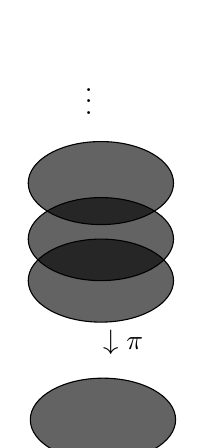
\begin{tikzpicture}[x=0.75pt,y=0.75pt,yscale=-1,xscale=1]
%uncomment if require: \path (0,300); %set diagram left start at 0, and has height of 300

%Shape: Ellipse [id:dp12336307762837184] 
\draw  [fill={rgb, 255:red, 0; green, 0; blue, 0 }  ,fill opacity=0.61 ] (285,236) .. controls (285,224.95) and (300.67,216) .. (320,216) .. controls (339.33,216) and (355,224.95) .. (355,236) .. controls (355,247.05) and (339.33,256) .. (320,256) .. controls (300.67,256) and (285,247.05) .. (285,236) -- cycle ;
%Shape: Ellipse [id:dp11661534507645899] 
\draw  [fill={rgb, 255:red, 0; green, 0; blue, 0 }  ,fill opacity=0.61 ] (284,169) .. controls (284,157.95) and (299.67,149) .. (319,149) .. controls (338.33,149) and (354,157.95) .. (354,169) .. controls (354,180.05) and (338.33,189) .. (319,189) .. controls (299.67,189) and (284,180.05) .. (284,169) -- cycle ;
%Shape: Ellipse [id:dp8216780422677058] 
\draw  [fill={rgb, 255:red, 0; green, 0; blue, 0 }  ,fill opacity=0.61 ] (284,149) .. controls (284,137.95) and (299.67,129) .. (319,129) .. controls (338.33,129) and (354,137.95) .. (354,149) .. controls (354,160.05) and (338.33,169) .. (319,169) .. controls (299.67,169) and (284,160.05) .. (284,149) -- cycle ;
%Shape: Ellipse [id:dp5707738774352155] 
\draw  [fill={rgb, 255:red, 0; green, 0; blue, 0 }  ,fill opacity=0.61 ] (284,122) .. controls (284,110.95) and (299.67,102) .. (319,102) .. controls (338.33,102) and (354,110.95) .. (354,122) .. controls (354,133.05) and (338.33,142) .. (319,142) .. controls (299.67,142) and (284,133.05) .. (284,122) -- cycle ;

% Text Node
\draw (310,67.4) node [anchor=north west][inner sep=0.75pt]    {$\vdots $};
% Text Node
\draw (326.6,191) node [anchor=north west][inner sep=0.75pt]  [rotate=-90]  {$\rightarrow $};
% Text Node
\draw (330,195.4) node [anchor=north west][inner sep=0.75pt]    {$\pi $};


\end{tikzpicture}
\end{figure}
\end{definition}
Let us begin with an important example.
\begin{example}
    Well, clearly, the easiest way to get a covering space out of any space is to simply consider that map $X\amalg X \to X$. But that's not interesting. \\
    The most important example of covering spaces that we will consider in this course is the exponential map:
    \begin{align*}
        \exp : \R &\longrightarrow S^1\\
        \theta&\longmapsto e^{2\pi i\theta}.
    \end{align*}
Let us make sure that this is indeed a covering map. Take any point $e^{2\pi i \theta} \in S^1$ where $0<\theta \le1$. Now consider an open set $U$ of $S^1$, formed by $B_\epsilon(e^{2\pi i \theta}) \cap S^1$ where $0< \epsilon <2$. Denote $U =: e^{2\pi i (\theta - \delta , \theta + \delta)}$ where clearly $0 <\delta <1/2$. Consider now $\pi^{-1}(U) \subseteq \R$. We will have 
    \begin{align*}
        \pi^{-1}(U) &= \coprod_{n\in \Z} (\theta +2\pi n-\delta , \theta + 2\pi n+ \delta).
    \end{align*}
    Denote $V_n:= (\theta + 2\pi n -\delta, \theta + 2\pi n+ \delta)$. Moreover, it is clear that 
    \begin{align*}
        \rest{\pi}{V_n} : V_n &\longrightarrow U
    \end{align*}
    is a homeomorphism. So indeed $\pi$ is a covering map of $S^1$. This is a very famous covering map as well. You should think of it as an infinite spiral (homeomorphic to $\R$) which covers the $S^1$ in the sense that when you view the spiral from the top, you will see only $S^1$. \\
    
    We will use this covering map $\exp : \R \to S^1$ to find the first homotopy group of $S^1$. The main idea there will be \textit{resolve} complicated loops in $S^1$ to $\R$, where each loop is homotopic to constant loop at the starting/ending point of the loop(!)
\end{example}
\begin{remark}
It is clear that every covering map is surjective.
\end{remark}
We have the following basic, but useful lemma.
\begin{lemma}\label{L-5.0.3}
Let $\pi : \tilde{X} \to X$ be a covering map. Then, for all $x\in X$ the fiber $\pi^{-1}(x) \subseteq \tilde{X}$ is a discrete subspace of $\tilde{X}$, that is, each $\tilde{x}\in \pi^{-1}(x)$ is both open and closed.
\end{lemma}
\begin{proof}
To see this, take any $\tilde{x}\in \pi^{-1}(x)$ and an evenly covered neighborhood $U_x \subseteq X$ of $x$. Since $\pi^{-1}(U_x) = \coprod_{\alpha \in J_x} V_\alpha$, where each $V_\alpha$ is homeomorphic to $U_x$ under $\rest{\pi}{V_\alpha}$. Thus, the unique ${\tilde x}_\alpha \in V_\alpha $ such that $\pi({\tilde x}_\alpha) = x$ is an element of $\pi^{-1}(x)$, one for each $\alpha \in J_x$. Now an open set of $\pi^{-1}(x)$ is of the form $V \cap \pi^{-1}(x)$ where $V\subseteq \tilde V$ is open, therefore $V_\alpha \cap \pi^{-1}(x)$ is open in $\pi^{-1}(x)$. But $V_\alpha \cap \pi^{-1}(x) = \{{\tilde x}_\alpha\}$ because each $V_\alpha$ are disjoint. Therefore $\{{\tilde x}_\alpha\}$ is open in $\pi^{-1}(x)$. Similarly, it is closed in $\pi^{-1}(x)$ by considering the complement of $\union_{\beta\neq \alpha} V_\beta$ in $\pi^{-1}(x)$. Hence $\pi^{-1}(x)$ is a discrete subspace of $\tilde{X}$.
\end{proof}
\subsection{Path lifting}
Covering maps are important in algebraic topology because they come equipped with a lot of unique lifting properties. We will first spell out the unique path lifting property of covering spaces, which is a baby version of unique homotopy lifting property. Before that, we need some specific property of a path in space $X$ which is covered by a covering space $\tilde X$.
\begin{lemma}\label{L-5.1.1}
Let $\gamma : I \to X$ be a path in $X$ and $\pi : \tilde{X} \to X$ be a covering map. Then there exists a partition $0 = t_0 < t_1 < t_2 < \dots < t_{k-1} < t_k = 1$ of unit interval $I$ such that for all $i=0,\dots,k-1$, the image $\gamma ([t_i,t_{i+1}])\subseteq X$ is contained in an evenly-covered neighborhood of $X$.
\end{lemma}
\begin{proof}
So first, for all $t\in I$, there exists an evenly-covered neighborhood $U_t \subseteq X$ of $\gamma(t) \in X$. Thus, by continuity of $\gamma$, we get that there exists $(a_t,b_t)\subseteq I$ containing $t\in I$ such that $\gamma((a_t,b_t))\subseteq U_t$. Since each open interval contains a compact interval, therefore we can assume $(a_t,b_t)$ to be $[a_t,b_t]$. So we have a family of closed subintervals $\{[a_t,b_t]\}_{t\in I}$ of $I$. By compactness of $I$, we get that there exists a finite subcover $[a_{t_1},b_{t_1}], \dots,[a_{t_n},b_{t_n}]$ of $I$. Now suppose $[a_{t_i},b_{t_i}]$ and $[a_{t_j},b_{t_j}]$ intersect, then we can break down $[a_{t_i},b_{t_i}]\cup [a_{t_j},b_{t_j}]$ into three disjoint closed intervals $[a_{t_i},a_{t_j}] \cup [a_{t_j},b_{t_i}] \cup [b_{t_i},b_{t_j}]$. Furthermore note that each of the above three have their images contained inside an evenly-covered neighborhood. Since there are only finitely many such intersections, therefore we have a finite disjoint cover of $I$ by closed intervals, each of which has image under $\gamma$ contained in an evenly covered neighborhood. 
\end{proof}
\begin{theorem}\label{T-5.1.2} (\textit{Unique path lifting of covering maps})
Let $\pi : \tilde{X} \to X$ be a covering map. Suppose there is a path $\gamma : I \to X$ and a prescribed point $\tilde{\gamma}_0 : \{0\} \to \tilde{X}$ such that $\pi(\tilde{\gamma}_0)= \gamma(0)$, then there exists a unique path $\tilde{\gamma} : I \to \tilde{X}$ such that $\pi \circ \tilde{\gamma} = \gamma$ and $\tilde{\gamma} (0) = \tilde{\gamma}_0$. That is, the following lifting problem is uniquely filled:
% https://q.uiver.app/?q=WzAsNCxbMCwwLCJcXHswXFx9Il0sWzAsMiwiSSJdLFsyLDIsIlgiXSxbMiwwLCJcXHRpbGRle1h9Il0sWzMsMiwiXFxwaSJdLFsxLDIsIlxcZ2FtbWEiLDJdLFswLDEsIiIsMix7InN0eWxlIjp7InRhaWwiOnsibmFtZSI6Imhvb2siLCJzaWRlIjoidG9wIn19fV0sWzAsMywiXFx0aWxkZXtcXGdhbW1hfV8wIiwwLHsic3R5bGUiOnsidGFpbCI6eyJuYW1lIjoiaG9vayIsInNpZGUiOiJ0b3AifX19XSxbMSwzLCJcXHRpbGRlXFxnYW1tYSIsMSx7InN0eWxlIjp7ImJvZHkiOnsibmFtZSI6ImRhc2hlZCJ9fX1dXQ==
\[\begin{tikzcd}
	{\{0\}} && {\tilde{X}} \\
	\\
	I && X
	\arrow["\pi", from=1-3, to=3-3]
	\arrow["\gamma"', from=3-1, to=3-3]
	\arrow[hook, from=1-1, to=3-1]
	\arrow["{\tilde{\gamma}_0}", hook, from=1-1, to=1-3]
	\arrow["\tilde\gamma"{description}, dashed, from=3-1, to=1-3]
\end{tikzcd}.\]
\end{theorem}
\begin{proof}
Let us first construct such a path lift. By Lemma \ref{L-5.1.1}, we have a partition of $I$ into $I = \cup_{i=0}^{k-1} [t_i,t_{i+1}]$ of disjoint closed intervals where $\gamma ([t_i,t_{i+1}])\subset U_i\subset X$ and $U_i$ is evenly-covered in $X$. Now to construct the said $\tilde{\gamma}$, we will have to do it for each $[t_i, t_{t+1}]$, starting from $i=0$, making use of $\tilde{\gamma}_0 \in \tilde{X}$ that has been already given to us. Now, let us first denote $\pi^{-1}(U_i) = \coprod_{\alpha \in J_i} V_\alpha^i$ for all $i=0, \dots, k-1$ where $V_\alpha^i \isom U_i$, which is given by the fact that $\pi$ is a covering map. Also keep in note that $\forall t\in [t_i,t_{i+1}]$, $\gamma(t)\in U_i\subseteq X$ which is evenly-covered.\\ 

So let us first define $\tilde \gamma $ for $[t_0, t_1] = [0,t_1]$. Since $\pi(\tilde{\gamma}_0) = \gamma (0) \in U_0$, therefore $\tilde{\gamma}_0 \in \pi^{-1}(U_0)$ and hence there is unique $\alpha_0 \in J_0 $ such that $\tilde{\gamma}_0 \in V_{\alpha_0}^0$.
\begin{align*}
    \rest{\tilde \gamma}{[t_0,t_1]} : [t_0, t_1] &\longrightarrow \tilde{X}\\
    t&\longmapsto \inv{\rest{\pi}{V^0_{\alpha_0}}}(\gamma(t)),
\end{align*}
where $\rest{\pi}{V^0_{\alpha_0}} : V^0_{\alpha_0} \to U_0$ is a homeomorphism and we are using it's inverse map in the above definition. Ok, so we first observe that $\rest{\tilde{\gamma}}{[t_0,t_1]}(0) = \inv{\rest{\pi}{V^0_{\alpha_0}}}(\gamma(0)) = \inv{\rest{\pi}{V^0_{\alpha_0}}}(\pi(\tilde{\gamma}_0)) = \tilde{\gamma}_0$. That is, the starting point of path $\tilde{\gamma}$ is indeed $\tilde{\gamma}_0$. So we have constructed a path in $\tilde{X}$ from $\tilde{\gamma}_0$ to $\rest{\tilde{\gamma}}{[t_0,t_1]}(t_1)$. Moreover, this path satsfies that $\pi \circ \rest{\tilde\gamma}{[t_0,t_1]} = \rest{\gamma}{[t_0,t_1]}$, which is exactly what we wanted. \\

Next, let us continue defining $\tilde\gamma$ for $[t_1,t_2]$ by using where we left off at $[t_0,t_1]$. This in turn will suggest us how to completely define the whole path $\tilde{\gamma}$. So we first note that $\gamma(t_1)\in U_0 \cap U_1$, therefore the end point of path $\rest{\tilde\gamma}{[t_0,t_1]}$ at $t_1$, takes value in $\pi^{-1}(U_1)$ as well, so let $\rest{\tilde\gamma}{[t_0,t_1]}(t_1) \in V^1_{\alpha_1} $. It should be clear by now what we are about to do; now define:
\begin{align*}
    \rest{\tilde\gamma}{[t_1,t_2]} : [t_1,t_2] &\longrightarrow \tilde{X}\\
    t &\longmapsto \inv{\rest{\pi}{V^1_{\alpha_1}}}(\gamma(t)).
\end{align*}
As usual, we again observe that $\rest{\tilde{\gamma}}{[t_1,t_2]} (t_1) = \rest{\tilde{\gamma}}{[t_0,t_1]}(t_1)$ because we have
\begin{align*}
    \inv{\rest{\pi}{V^1_{\alpha_1}}}(\gamma(t_1)) &= \inv{\rest{\pi}{V^1_{\alpha_1}}}(\pi(\rest{\tilde{\gamma}}{[t_0,t_1]}(t_1) ))\\
    &= \rest{\tilde{\gamma}}{[t_0,t_1]}(t_1)
\end{align*}
where we conclude second line from first as $\gamma(t_1) \in U_0\cap U_1$, where $\inv{\rest{\pi}{V^1_{\alpha_1}}}$ is indeed defined. So we have indeed define a path $\rest{\tilde{\gamma}}{[t_1,t_2]}$ whose starting point is same as the ending point of $\rest{\tilde\gamma}{[t_0,t_1]}$, so we have defined the $\tilde\gamma$ upto $[t_0,t_2]$. \\

Having done the above, we now give general procedure of continuing the definition of path $\tilde\gamma$ till $[t_{k-1}, t_k]$. Suppose $2\le j\le k-1$ and suppose we have constructed  $\rest{\tilde\gamma}{[t_{j-1},t_j]} : [t_{j-1},t_j] \to \tilde{X}$ as of yet. So we know the point $\rest{\tilde\gamma}{[t_{j-1}, t_j]}(t_j)\in V^{j-1}_{\alpha_{j-1}}$ where $ \gamma(t_j)\in U_{j-1} \cap U_j$. We now construct with this information the next piece of path $\rest{\tilde\gamma}{[t_{j}, t_{j+1}]} : [t_j,t_{j+1}] \to \tilde{X}$. Well, the following definition shouldn't be a surprise:
\begin{align*}
    \rest{\tilde\gamma}{[t_j,t_{j+1}]} : [t_j,t_{j+1}] &\longrightarrow \tilde{X}\\
    t&\longmapsto \inv{\rest{\pi}{V^j_{\alpha_j}}}(\gamma(t))
\end{align*}
where we again observe that the starting point of the above path is same as $\rest{\tilde\gamma}{[t_{j-1}, t_j]}(t_j)$. Moreover, it is easy to observe that $\pi\circ \rest{\tilde\gamma}{[t_j,t_{j+1}]}= \rest{\gamma}{[t_j,t_{j+1}]}$.\\

Finally, since there are only finitely many $[t_j,t_{j+1}]$s, therefore we have constructed a path $\tilde\gamma$ in $\tilde X$ such that it starts from $\tilde{\gamma}_0$ ($\tilde{\gamma}_0 = \tilde{\gamma}(0)$) and when projected back to $X$ under $\pi$, we obtain the path $\gamma $ back ($\pi \circ \tilde \gamma = \gamma$). In particular, the end point $\tilde\gamma (1)\in \pi^{-1}(\gamma(1))$. The uniqueness of $\tilde{\gamma}$ follows by construction.
\end{proof}
\subsection{Homotopy lifting}
The Theorem \ref{T-5.1.2} will be the building block for it's generalization, which is the homotopy lifting of covering maps. Let us first define what does it mean for a map to have homotopy lifting property.
\begin{definition}
(\textbf{Homotopy lifting property}) Let $p : E\to B$ be a continuous map. The map $p$ is said to have homotopy lifting property if for any homotopy $H : Y\times I \to B$ and any map $\tilde{H}_0 : Y\times \{0\} \to E$ such that $p \circ \tilde{H}_0 = H(-, 0)$, there exists a homotopy $\tilde H : Y\times I \to E$ such that $\tilde{H}(-,0) = \tilde{H}_0$ and $p\circ \tilde{H} = H$. That is, the following lifting problem is filled:
% https://q.uiver.app/?q=WzAsNCxbMCwwLCJZXFx0aW1lc3swfSJdLFswLDIsIllcXHRpbWVzIEkiXSxbMiwwLCJFIl0sWzIsMiwiQiJdLFsxLDMsIkgiLDJdLFsyLDMsInAiXSxbMCwxLCIiLDAseyJzdHlsZSI6eyJ0YWlsIjp7Im5hbWUiOiJob29rIiwic2lkZSI6InRvcCJ9fX1dLFswLDIsIlxcdGlsZGV7SH1fMCJdLFsxLDIsIlxcdGlsZGV7SH0iLDEseyJzdHlsZSI6eyJib2R5Ijp7Im5hbWUiOiJkYXNoZWQifX19XV0=
\[\begin{tikzcd}
	{Y\times{0}} && E \\
	\\
	{Y\times I} && B
	\arrow["H"', from=3-1, to=3-3]
	\arrow["p", from=1-3, to=3-3]
	\arrow[hook, from=1-1, to=3-1]
	\arrow["{\tilde{H}_0}", from=1-1, to=1-3]
	\arrow["{\tilde{H}}"{description}, dashed, from=3-1, to=1-3]
\end{tikzcd}.\]
\end{definition}
\begin{remark}
It is clear that path lifting property is obtained from homotopy lifting property by setting $Y = \{0\}$ in the diagram of homotopy lifting problem above.
\end{remark}
We then have the following theorem.
\begin{theorem}\label{T-5.2.3}
(\textit{Unique homotopy lifting of covering maps}) Let $\pi : \tilde{X} \to X$ be a covering map. Then $\pi$ satisfies unique homotopy lifting property. That is, given any homotopy $H : Y\times I \to X$ and a map $\tilde{H}_0 : Y\to \tilde{X}$ such that $\pi \circ \tilde{H}_0 = H(-,0)$, there exists a unique homotopy $\tilde{H} : Y\times I \to \tilde{X}$ such that $\tilde{H}(-,0) = \tilde{H}_0$ and $\pi \circ \tilde{H} = H$. In other words, the following lifting problem is uniquely filled:
% https://q.uiver.app/?q=WzAsNCxbMCwyLCJZXFx0aW1lcyBJIl0sWzAsMCwiWVxcdGltZXMgXFx7MFxcfSJdLFsyLDIsIlgiXSxbMiwwLCJcXHRpbGRle1h9Il0sWzMsMiwiXFxwaSJdLFswLDIsIkgiLDJdLFsxLDAsIiIsMix7InN0eWxlIjp7InRhaWwiOnsibmFtZSI6Imhvb2siLCJzaWRlIjoidG9wIn19fV0sWzEsMywiXFx0aWxkZXtIfV8wIl0sWzAsMywiXFx0aWxkZXtIfSIsMSx7InN0eWxlIjp7ImJvZHkiOnsibmFtZSI6ImRhc2hlZCJ9fX1dXQ==
\[\begin{tikzcd}
	{Y\times \{0\}} && {\tilde{X}} \\
	\\
	{Y\times I} && X
	\arrow["\pi", from=1-3, to=3-3]
	\arrow["H"', from=3-1, to=3-3]
	\arrow[hook, from=1-1, to=3-1]
	\arrow["{\tilde{H}_0}", from=1-1, to=1-3]
	\arrow["{\tilde{H}}"{description}, dashed, from=3-1, to=1-3]
\end{tikzcd}.\]
\end{theorem}
\begin{proof}
\textbf{[TODO] Proof is quite long and detailed so I will do it when I will get time.}.
\end{proof}
\subsection{$\pi_1(S^1) \isom \Z$}
We now prove using the covering map $\exp : \R \to S^1$ that the first homotopy group of $S^1$ is $\Z$.
\begin{theorem}
$\pi_1(S^1) \isom \Z$.
\end{theorem}
\begin{proof}
Consider the following map which is quite intuitive to define:
\begin{align*}
    \varphi :  \Z &\longrightarrow \pi_1(S^1)\\
    n&\longmapsto [\gamma_n]
\end{align*}
where $\gamma_n : I\to S^1$ is the loop $\theta\longmapsto e^{2\pi i n \theta }$, that is, $\gamma_n$ is the loop corresponding to travelling around $n$-times on the circle $S^1$. Let us first show that it is indeed a group homomorphism. We see that
\begin{align*}
    \varphi(n+m)&= [\gamma_{n+m}]\\
    &= [\gamma_n *\gamma_m]\\
    &= [\gamma_n]*[\gamma_m]\\
    &= \varphi(n)*\varphi(m),
\end{align*}
so no qualms there. \\

The major hurdle starts when we try to prove the injectivity and surjectivity. This is where we will need to use the path and homotopy lifting properties of the covering map $\exp : \R \to S^1$ where we indeed verified that $\exp$ is a covering map in the example below the definition of covering spaces.\\

Let us first show surjectivity. So take any $[\gamma]\in \pi_1(S^1)$. We need to show that $\exists n\in \Z$ such that $[\gamma_n] = [\gamma]$. So we have that $\exp(\tilde{x}) = \gamma_n(0)$, which in diagrammatic form is
% https://q.uiver.app/?q=WzAsNCxbMCwyLCJJIl0sWzIsMiwiU14xIl0sWzIsMCwiXFxSIl0sWzAsMCwiXFx7MFxcfSJdLFszLDAsIiIsMCx7InN0eWxlIjp7InRhaWwiOnsibmFtZSI6Imhvb2siLCJzaWRlIjoidG9wIn19fV0sWzMsMiwiXFx0aWxkZXt4fSIsMCx7InN0eWxlIjp7InRhaWwiOnsibmFtZSI6Imhvb2siLCJzaWRlIjoidG9wIn19fV0sWzIsMSwiXFxleHAiXSxbMCwxLCJcXGdhbW1hIiwyXV0=
\[\begin{tikzcd}
	{\{0\}} && \R \\
	\\
	I && {S^1}
	\arrow[hook, from=1-1, to=3-1]
	\arrow["{\tilde{x}}", hook, from=1-1, to=1-3]
	\arrow["\exp", from=1-3, to=3-3]
	\arrow["\gamma"', from=3-1, to=3-3]
\end{tikzcd}.\]
Since $\exp: \R\to S^1$ is a covering map, therefore using the unique path lifting property of covering maps (Theorem \ref{T-5.1.2}), we get that there is a unique $\tilde{\gamma} : I\to \R$ such that the above lifting problem is filled and then we get $\exp\circ \tilde{\gamma} = \gamma$ and $\tilde{\gamma}(0) = \tilde{x} \in \inv{\exp}(1)$. Now, we also have that $\tilde{\gamma}(1) \in \inv{\exp}(1)$. Therefore $\tilde{\gamma}(1) - \tilde{\gamma}(0) = $ total number of times the loop $\gamma$ crosses 1 = $n$, say. So $\tilde{\gamma}$ is homotopic to the straight line joining $\tilde{\gamma}(0)$ and $\tilde{\gamma}(1)$, that is $\kappa(t) = (1-t)\tilde{\gamma}(0) + t\tilde{\gamma}(1)$. Let this homotopy between $\kappa $ and $\tilde{\gamma}$ be denoted by $H : I\times I \to \R$. Then $\exp \circ H$ is a homotopy between $\exp \circ \kappa$ and $\exp \circ \tilde{\gamma}$ where the former is the $\gamma_n$ and the latter is $\gamma$. We thus have a homotopy between them and therefore $[\gamma]= [\gamma_n]$.\\

Let us next show injectivity. So suppose $\varphi(n)  =[\gamma_n] =[c_1] = [\gamma_0]$ where $c_1 = \gamma_0 : I \to S^1$ is the constant loop at $1\in S^1$. We need to show that this implies $n=0$. We will use homotopy lifting to prove this, that is, we will lift the homotopy which makes $\gamma_n$ homotopic to $c_1$ to a homotopy in $\R$ between the lift of $\gamma_n$ to a constant path. More precisely, consider the homotopy 
\begin{align*}
    H: I \times I &\longrightarrow S^1
\end{align*}
establishing a homotopy between $H(-,0) = \gamma_n$ and $H(-,1) = \gamma_0$ and moreover $H(0,-) = H(1,-) = 1$. Also consider the map $\tilde{\gamma}_n : I \longrightarrow \R$ given by $t \longmapsto nt$. This is the other map which the lifted homotopy will give a homotopy from to some other map (which we have to figure out). We then observe that $\tilde{\gamma}_n$ is the right map to define here because $\exp \circ \tilde{\gamma}_n(s) = e^{2\pi i ns} = \gamma_n(s) = H(s,0)$. Ok so now we lift. Using Theorem \ref{T-5.2.3}, the following lifting problem is uniquely solved:
% https://q.uiver.app/?q=WzAsNCxbMCwyLCJJXFx0aW1lcyBJIl0sWzIsMiwiU14xIl0sWzIsMCwiXFxSIl0sWzAsMCwiSVxcdGltZXNcXHswXFx9Il0sWzAsMSwiSCIsMl0sWzIsMSwiXFxleHAiXSxbMywwLCIiLDIseyJzdHlsZSI6eyJ0YWlsIjp7Im5hbWUiOiJob29rIiwic2lkZSI6InRvcCJ9fX1dLFszLDIsIlxcdGlsZGV7XFxnYW1tYX1fbiJdLFswLDIsIlxcdGlsZGV7SH0iLDEseyJzdHlsZSI6eyJib2R5Ijp7Im5hbWUiOiJkYXNoZWQifX19XV0=
\[\begin{tikzcd}
	{I\times\{0\}} && \R \\
	\\
	{I\times I} && {S^1}
	\arrow["H"', from=3-1, to=3-3]
	\arrow["\exp", from=1-3, to=3-3]
	\arrow[hook, from=1-1, to=3-1]
	\arrow["{\tilde{\gamma}_n}", from=1-1, to=1-3]
	\arrow["{\tilde{H}}"{description}, dashed, from=3-1, to=1-3]
\end{tikzcd}.\]
So we have a homotopy $\tilde{H} : I\times I \longrightarrow \R$ such that $\tilde{H}(s,0) = \tilde{\gamma}_n(s)$ and, more importantly, $\exp \circ \tilde{H} = H$. Thus, $\exp (\tilde{H}(s,1)) = H(s,1) = 1$, that is, $\Image{ \tilde{H}(-,1)} \subseteq \inv{\exp }(1)$. Since fibres of a covering map are necessarily discrete (Lemma \ref{L-5.0.3}) and $\tilde{H}(-,1)$ is a continuous map from a connected set $I$, so it's image has to be connected as well and hence $\Image{\tilde{H}(-,1)}$ has to be a point inside $\inv{\exp}(1)$. What this means is that $\tilde{H}(-,1)$ is a constant map, to a point in $\R$, which we denote as $a\in \R$ such that $\exp (a) =1$. So $\tilde{H}$ is a homotopy between $\tilde{\gamma}_n$ and $c_a$ (the constant path at $a$). Moreover, we also have that $\tilde{H}(0,t)= \tilde{H}(1,t) $ for all $t\in I$ because $\tilde{H}$ is a based homotopy. So we get that the map $\tilde{H}(1,t) = \tilde{H}(0,t) = a \in \inv{\exp}(1)$ for all $t\in I$ as it is $a$ for $t=1$. So this \textbf{forces} $\tilde{H(s,0)} =\tilde{\gamma}_n(s) $ to have starting point and ending point same, equal to $a$. But this can only happen when $n=0$ (see definition of $\tilde{\gamma}_n$). We are done.
\end{proof}
\subsection{Couple of properties of covering spaces}
Covering maps are quite nice maps as is shown by Theorem \ref{T-5.2.3}. We will consider a couple of important properties that covering spaces hold in this section. The first one being that all fibers of a covering map of a path-connected space (which is discrete, Lemma \ref{L-5.0.3}) are bijective (so have same \textit{size}).
\begin{lemma}
Let $\pi : \tilde{X} \to X$ be a covering map and let $X$ be a path-connected space\footnote{or work over path-components.}. Let $x_0,x_1\in X$ be two points, then there is a set bijection
\begin{align*}
    \pi^{-1} (x_0) \isom     \pi^{-1}(x_1).
\end{align*}
\begin{proof}
\textbf{[TODO]}.
\end{proof}
\end{lemma}
Another use of covering spaces is that if $\pi : \tilde{X} \to X$ is a covering map where both the spaces are path-connected, then the fundamental group of $\tilde{X}$ is naturally embedded inside the fundamental group of $X$.
\begin{proposition}
Let $\pi : \tilde{X} \to X$ be a covering map where both $X$ and $\tilde{X} $ are path-connected. Then the map 
\begin{align*}
    \pi_1(\pi) : \pi_1(\tilde{X},\tilde{x}_0) &\longrightarrow \pi_1(X,\pi(\tilde{x}_0))
\end{align*}
is injective.
\end{proposition}
\begin{proof}
    \textbf{[TODO]}.
\end{proof}
\newlecture{12}{02/09/2022}
\subsection{Fun applications of $\pi_1(S^1) \isom \Z$}
We first have the famous Brouwer's fixed point theorem.
\begin{proposition}
(\textit{Brouwer's fixed point theorem}) For any continuous $f : D^2 \to D^2$, there exists a point $x\in D^2$ such that $f(x) = x$.
\end{proposition}
\begin{proof}
\textbf{[TODO]}.
\end{proof}
Next is something we know very well but didn't knew that it can be done from the methods we have developed till now:
\begin{proposition}
(\textit{Fundamental theorem of algebra}) Let $p(x) \in \mathbb{C}[x]$. Then there exists a $c\in \mathbb{C}$ such that $x-c$ divides $p(x)$. That is, every complex polynomial has a root in $\mathbb{C}$ (and thus have all roots in $\mathbb{C}$).
\end{proposition}
\begin{proof}
\textbf{[TODO]}.
\end{proof}
The last one is something we saw in the departmental seminar a week ago, using which we saw that one can prove very non-trivial combinatorial results.
\begin{proposition}
(\textit{Borsuk-Ulam theorem}) If $f : S^2 \to \R^2$ is a continuous map, then there exists a pair of anti-podal points which are mapped to same point under $f$.
\end{proposition}
\begin{proof}
\textbf{[TODO]}.
\end{proof}
\newlecture{13}{06/09/2022}
\begin{center}
    \scshape{{Class Test - 1}}
\end{center}
\newlecture{14}{14/09/2022}
\begin{center}
    \scshape{Mid-Semester Evaluation}
\end{center}
%\newpage
%\section{The Van-Kampen theorem}
%lol no. \textbf{[TODO]} Maybe I'll do what May did in his notes and call it a day.
\newpage
\newlecture{15}{20/09/2022}
\section{Covering spaces, group actions and Galois theory of covers}
So in this second phase of the course, we will be seeing some more fancy theorems, but the main goal will be to go to some calculative things, like computing homology groups and all that. In any case, we covered covering spaces, but it would be rather incomplete if we don't say something about universal covering and more theorems in that direction. The first theorem we therefore discuss, tells us how a certain type of $G$-space naturally enriches the quotient map with the structure of a covering space. We first define the type of $G$-space we wish to look out for.
\begin{definition}
(\textbf{Properly discontinuous action}) Let $G$ be a group and $X$ be a space with a continuous action\footnote{this means that the action map $G\times X \to X$ is a continuous map where $G$ is given the discrete topology.} of $G$. The action of $G$ is said to be properly discontinuous if for all $x\in X$, there exists an open set $U_x \subseteq X$ containing $x$ such that $gU_x \cap U_x = \emptyset$ for all $g\in G$.
\end{definition}
There is another type of action:
\begin{definition}
(\textbf{Free action}) Let $G$ be a group acting continuously on space $X$. The the action is said to be free if for all $x\in X$, the stabilizer subgroup is trivial, that is, $S_G(x) = \{e\}$.
\end{definition}
There are some consequences of the above definition which we collectively state in the the following lemma:
\begin{lemma}\label{L-6.0.3}
Let $G$ be a group and $X$ be a space with continuous $G$-action.
\begin{enumerate}
    \item{If the action is properly discontinuous, then it is free.}
    \item{If $G$ is finite and $X$ is locally finite\footnote{this means that for all $x\in X$, there exists a sequence of open sets $U_n$ containing $x$ such that $\bigcap_n U_n = \{x\}$.}, then the action is free if and only if it is properly discontinuous.}
\end{enumerate}
\end{lemma}
\begin{proof}
1. Take any $x\in X$. Let $U_x$ be the open set containing $x$ obtained from properly discontinuous action of $G$. If $g\in S_G(x)$, then $gU_x \cap U_x \neq \emptyset$. Thus $g=e$.\\

2. R $\Rightarrow$ L is simple. For L $\Rightarrow$ R, we go by contradiction. So suppose the action is free but not properly discontinuous. Take any point $x\in X$. So for any open $U \ni x$ and for any $g\in G$, $gU \cap U \neq \emptyset$. Now, we have a sequence of open sets each containing $x$, $U_n$, such that $\cap_{n}U_n = \{x\}$. Since $gU_n \cap U_n \neq \emptyset$ for each $n$, therefore we get a sequence $\{x_n\}$ where $x_n \in U_n$ such that $\lim x_n = x$ and $\lim gx_n = x$. Since $g\in G$ can be treated as $g  : X\to X$ a homeomorphism, therefore $g(\lim x_n) = x $ that is $gx = x$, a contradiction to the fact that $G$ acts freely\footnote{this is in-line with what the wonderful man \textit{I.P. Freely} had to say.}.  
\end{proof}
Let us now state the theorem of interest.
\begin{theorem}\label{T-6.0.4} Let $G$ be a group and $X$ be a space with continuous $G$-action. If the action is properly discontinuous, then the quotient map 
% https://q.uiver.app/?q=WzAsMixbMCwwLCJxIDpYIl0sWzEsMCwiWC9HIl0sWzAsMSwiIiwwLHsic3R5bGUiOnsiaGVhZCI6eyJuYW1lIjoiZXBpIn19fV1d
\[\begin{tikzcd}
	{q :X} & {X/G}
	\arrow[two heads, from=1-1, to=1-2]
\end{tikzcd}\]
is a covering map.
\end{theorem}
Before stating the proof, we would like to give some example uses of this theorem.
\begin{example}
Consider $G = \mathbb{Z}^n$ and $X = \mathbb{R}^n$. There is a canonical action we can define on $\mathbb{R}^n$ using $\mathbb{Z}^n$ given by 
\begin{align*}
    G\times X &\longrightarrow X\\
    ((m_1,\dots,m_n),(x_1,\dots,x_n)) &\longmapsto (m_1+x_1, \dots, m_n + x_n).
\end{align*}
The fact that this is a continuous action is trivial to check. We first claim that this action is properly discontinuous. It is simple to see why that's the case; for an $x\in X$ simply take any $0<a<1/2$ and define $U = \prod (x_i-a,x_i+a)$. This $U$ is open and for any $m:=(m_1,\dots,m_n)\in \mathbb{Z}^n$, $(m + U )\cap U = \emptyset$ for any $m\neq 0$. So indeed the action is properly discontinuous.\\

Next, we observe that $X/G = \mathbb{R}^n/\mathbb{Z}^n$ is simply homeomorphic to $[0,1]^n/G$ and which is in turn homeomorphic to $\left([0,1]/0\sim 1\right)^n$ and which is just $(S^1)^n$. So that is why the questions regarding $\R/\Z$ are so innumerable in literature, as they quickly form spaces which are quite weird to imagine. 
\end{example}
\begin{example}
(\textit{Configuration space of $k$-points in space $X$}) Let $X$ be a space. The configuration space of $k$ points in $X$, denoted $F_k(X)$, is intuitively the set of all possible positions that $k$ particles moving in $X$ can inhabit. More precisely, we define:
\begin{align*}
    F_k(X) = \{(x_1,\dots,x_k) \in \prod_{i=1}^k X\;\vert\; \forall \;i\neq j = 1,\dots,k, \; x_i \neq x_j \}.
\end{align*}
This space has an action of $S_k$, the symmetry group of $k$ letters, given by:
\begin{align*}
    S_k\times F_k(X) &\longrightarrow F_k(X)\\
    (\sigma, x_1,\dots,x_k) &\longmapsto (x_{\sigma(1)},\dots,x_{\sigma(k)}).
\end{align*}
In other words, we just permute the $k$ points which we find in some position in $X$. For $k=2$, we get that since $S_2 = \Z_2$, so the only action possible is
\begin{align*}
    \Z_2 \times F_2(X) &\longrightarrow F_2(X)\\
    (0,x_1,x_2) &\longmapsto (x_1,x_2)\\
    (1,x_1,x_2)&\longmapsto (x_2,x_1).
\end{align*}
In other words, we swap the two points. Then, orbits of the action of $\Z_2$ over $F_2(X)$ will consist of just the point itself and it's swapped counterpart. Hence, 
\begin{align*}
    F_2(X)/\Z_2 \isom (X\times X) / \sim
\end{align*}
where $(x_1,x_2) \sim (y_1,y_2)$ iff $x_1=y_2$ and $x_2 = y_1$. To better understand the situation, suppose $X= S^1$. Then, $F_2(S^1) = S^1\times S^1/ \sim$. Since $S^1  \times S^2 = T^2$, therefore we get $F^2(S^1) = T^2  \setminus \Delta (S^1)$, where $\Delta(S^1)$ is the diagonal subspace of $S^1\times S^2$. But $T^2\setminus \Delta(S^1)$ will look like quotient of $I\times I \setminus \Delta(I) $ which looks like two disjoint right triangles together. Now, we can obtain $F_2(S^1)/\sim$ by identifying the two triangles and doing the ensuing identifications of $I\times I$ to reach some weird object. 
\end{example}
\newlecture{16}{22/09/2022}
\begin{example}
	The next example that we do is known for it's weirdness. It is the construction of \textit{lens space}. Consider the odd sphere $ S^{2k+1} \subset \mathbb{C}^{k+1}$ for $ k \in \mathbb{N}$. Consider the cyclic group $ \Z_d $ where we take the following presentation of it: $ \Z_d =  \gen{\xi}$ where $ \xi $ is the $ d^\text{th} $ root of unity. We then have the following action of $ \Z_d $ on $ S^{2k+1} $:
	\begin{align*}
		\Z_d \times S^{2k+1} &\longrightarrow S^{2k+1}\\
		(\xi,z_1,\dots,z_k) &\longmapsto (\xi z_1,\dots,\xi z_k).
	\end{align*}
	This is indeed a valid action. In particular, we claim that this is a free action so that by Lemma \ref{L-6.0.3}, 2, this action becomes properly discontinuous and we can then use Theorem \ref{T-6.0.4} to get that $ S^{2k+1} $ is a cover of this so-called lens space. To see that it is free, take any $ (z_1,\dots,z_k) \in S^{2k+1} $. We see that if $ (\xi^n z_1,\dots,\xi^n z_k) = (z_1,\dots,z_k) $, then $ \xi^n = 1 $. So each stabilizer subgroup is trivial. Hence the action is free. Then, the lens space is defined to be the quotient $ S^{2k+1}/\Z_d $. Whatever that may look like, it has a structure of a $ 2k+1 $ dimension manifold, as we have a cover by Theorem \ref{T-6.0.4}.
\end{example}
With all these examples out of the way, let us now get to the proof of the theorem at hand.
\begin{proof}[Proof of Theorem \ref{T-6.0.4}]
	Since the action of $ G $ is properly discontinuous, therefore for each $ x\in X $, there exists open $ U_{x} \subseteq X $ such that $ gU_x \cap U_{x} = \emptyset $ for all $ g\in G $. We claim that for any $ [x]\in X/G $, the set $ V_x := q(U_x) $ is evenly covered open neighborhood of $ [x] $. In order to show this, we first claim the following
	\begin{align*}
		q^{-1}(V_x) = \coprod_{g\in G} gU_x.
	\end{align*}
	Now, since $ g :X\to X $ is a homeomorphism, thus $ gU_x = g(U_{x}) \subseteq X$ is open in $ X $. Hence, $ q^{-1}(V_x) $ is open in $ X $, if the above claim is true. So in order to see the claim, we see that
	\begin{align*}
		q^{-1}(V_x) &= \{y\in X\;\vert\; q(y) \in V_x = q(U_x)\}\\
		&= \{y\in X\;\vert\; \exists z\in U_x \text{ s.t. } q(y) = q(z)\}\\
		&= \{y\in X\;\vert\; \exists z\in U_x \text{ s.t. } y = gz \text{ for some }g\in G\}\\
		&= \bigcup_{g\in G} gU_x.
	\end{align*}
	So we need only show that $ gU_x \cap hU_x = \empty $. This is simple because if it is not the case, then for some $y,z\in U_x  $, we get $ gy = hz $, so $ y = g^{-1}hz $, a contradiction to $ U_x \cap g^{-1}h U_x = \emptyset $ by properly discontinuous action of $ G $ on $ X $. So indeed the claim is true. \\
	
	We need only show now that for any $ g\in G $, the restriction
	\begin{align*}
		\rest{q}{gU_x} : gU_x &\longrightarrow V_x
	\end{align*}
 	is a homeomorphism. Firstly, it is rather easy to see that $ q(gU_x) = q(U_x) $, after all, $ q $ kills all orbits so that $ q(gy) = q(y) $. Next, since $ q(U_x) =: V_x $, so the above map is well defined. We now only need to show that it is a homeomorphism. For that, we can consider the following inverse:
 	\begin{align*}
 		w : V_x := q(U_x) &\longrightarrow gU_x\\
 			q(y) &\longmapsto gy.
 	\end{align*}
 	This is indeed well-defined. To see this, take any $ z\in U_x $ such that $ q(y) = q(z) $. Thus there is an $ h\in G $ such that $ y = hz $. Since $ y,z\in U_x $ and $ U_x $ is such that $ kU_x \cap U_x = \emptyset \;\forall k\in G$, thus, if $ q(y) = q(z) $, then $ y=z $, hence $ gy=gz $. It is now easy to see that $ w $ is a continuous inverse of $ \rest{q}{gU_x} $, as $ gy\mapsto q(gy) \mapsto w(q(gy)) = gy $ and conversely $ q(y) \mapsto gy \mapsto q(gy) = y $. This completes the proof.
\end{proof}
\newlecture{17}{23/09/2022}
\subsection{Category of covering maps}
Let $ (X,x_{0})$ be a based space. It is easy to see that knowing information about all covers of $ (X,x_{0}) $, would be pretty handy. But how can one do that? Well, we will try to do exactly that in this section. Since we want to handle all covers of $ X $, so it is better we start giving this collection of all covers of $ (X,x_{0}) $ some structure. One structure that it has is that it forms a category.
\begin{definition}\label{D-6.1.1}
	(\textbf{The category $ \Cov{X,x_0} $})	Let $ (X,x_0) $ be a based map. The category of covering maps of $ (X,x_0) $ and homomorphisms between them is defined by:
	\begin{enumerate}
		\item {\textbf{Objects}: An object of $ \Cov{X,x_0} $ is a covering map $ p : (\tilde{X},\tilde{x}_0) \to (X,x_0)$.}
		\item {\textbf{Arrows}: An arrow in $ \Cov{X,x_0} $ is a continuous based map $ f : (\tilde{X}_1,\tilde{x}_1) \to (\tilde{X}_2,\tilde{x}_2)$ such that the following commutes:
	% https://q.uiver.app/?q=WzAsMyxbMCwwLCIoXFx0aWxkZXtYfV8xLFxcdGlsZGV7eH1fMSkiXSxbMiwwLCIoXFx0aWxkZXtYfV8yLFxcdGlsZGV7eH1fMikiXSxbMSwxLCIoWCx4XzApIl0sWzAsMiwicF8xIiwyXSxbMSwyLCJwXzIiXSxbMCwxLCJmIl1d
	\[\begin{tikzcd}
		{(\tilde{X}_1,\tilde{x}_1)} && {(\tilde{X}_2,\tilde{x}_2)} \\
		& {(X,x_0)}
		\arrow["{p_1}"', from=1-1, to=2-2]
		\arrow["{p_2}", from=1-3, to=2-2]
		\arrow["f", from=1-1, to=1-3]
	\end{tikzcd}.\]	
	}
	\end{enumerate}
\end{definition}
It is clear that $ \Cov{X,x_0} $ is a sub-category of the category $ \cat{Top}_* $ over $ (X,x_0) $, that is, $ \Cov{X,x_0} \subseteq \cat{Top}_*/(X,x_0) $. \\

We will see in this and the following sections that the main ingredient of our goal to understand a covering space will be, just like in Galois theory, the automorphism group of $ (\tilde{X},\tilde{x}_0) $ in the category $ \Cov{X,x_0} $. We denote the set of all \textbf{automorphisms} of $ (\tilde{X},\tilde{x}_0) $ by $ \Deck{\tilde{X},x_0} $. Note that in the unbased setting, we will denote the automorphism group of $ \tilde{X} \in \Cov{X,x_0}$ as just $ \Deck{X} $. \\

From now, we will abbreviate a based space $ (X,x_0) $ by just $ X $. Similarly for the covering spaces.\\

For our purposes, we see the following result.
\begin{proposition}\label{P-6.1.12}
	Let $ X $ be a path connected and locally path connected based space and consider $ (\tilde{X}_1,p_1) $ and $ (\tilde{X}_2,p_2) $ to be two path-connected covers in $ \Cov{X} $. Let $ \varphi: (\tilde{X}_1,p_1) \to (\tilde{X}_2,p_2) $ be a map of covering spaces. Then, $ \varphi $ is a covering map over $ (\tilde{X}_2,p_2) $. 
\end{proposition}
\begin{proof}We break the proof into following steps.
	\begin{act}{1}{The map $ \varphi $ is surjective.}
		Take any point $ y\in \tilde{X}_2 $. Since $ \tilde{X}_2 $ is path connected, so there is a path $ \eta : I \to \tilde{X}_2 $ with $ \eta(0) = \tilde{x}_2 $ and $ \eta(1) = y $. Then we have $ z:= p_2(y) \in X  $. Since $ X $ is path-connected, we thus have a path $ \gamma : I\to X $ such that $ \gamma(0) = x_0 $ and $ \gamma(1) = z $. By Theorem \ref{T-5.1.2} on $ \tilde{X}_2 $, it can be easily seen that $ \eta $ is the unique lift of $ \gamma $. Now, by Theorem \ref{T-5.1.2} for covering space $ \tilde{X}_1 $ with starting point $ \tilde{x}_1 $, we get a path $ \tilde{\gamma}_1 : I\to \tilde{X}_1 $ such that $ \tilde{\gamma}_1(0) = \tilde{x}_1 $ and $ p_1\circ \tilde{\gamma}_1 = \gamma $. Moreover, it is unique w.r.t. these properties. Now denote $ x:= \tilde{\gamma}_1(1) \in \tilde{X}_1$. Now, we have another path $\tilde{\gamma}_2 := \varphi\circ \tilde{\gamma}_1 : I\to \tilde{X}_2$ such that $ \tilde{\gamma}_2(0) = \tilde{x}_2 $. Moreover, by the fact that $ p_2\circ \varphi = p_1 $, we get that $ p_2\circ \tilde{\gamma}_2 = \gamma $. So if we apply Theorem \ref{T-5.1.2} on $ \tilde{X}_2 $, then the path that we must get should exactly be $ \tilde{\gamma}_2 $ because it satisfies the conditions that makes the path coming from the theorem unique. But then, $ \eta = \tilde{\gamma}_2 $. Hence $ \tilde{\gamma}_2(1) = \eta(1) = y $. Hence $ \varphi(x) = y $. This completes Act 1.
	\end{act}
	\begin{act}{2}{Each point of $ \tilde{X}_2 $ has an evenly covered neighborhood.}
		Take any point $ y\in \tilde{X}_2 $. To get an evenly covered neighborhood of $ y $, we begin with $ z:= p_2(y) \in X$. Since both $ \tilde{X}_1,\tilde{X}_2 $ are covering $ X $, therefore there are evenly covered neighborhoods $ U_1,U_2 \subseteq X $ containing $ z $. Then $ V:= U_1\cap U_2 $ is an open set which is an evenly covered neighborhood for both the covers. Now, $ \inv{p_2}(V) \ni y $. Since $ \inv{p_2}(V) = \coprod_{i\in J_z} V_i $. Let $ y\in V_{i_y} $. We claim that this $ V_{i_y} $ will be an evenly covered neighborhood of $ y\in \tilde{X}_2 $ for $ \varphi $. Clearly, $ \inv{\varphi}(V_{i_y}) \isom \inv{p}(V) \isom \coprod_{i\in I_z} W_i$ where $ \rest{p_1}{W_i} : W_i \to V $ which is a homeomorphism. This concludes Act 2.
	\end{act}
	This concludes the proof.
\end{proof}
We now define universal covering space of a based space.
\begin{definition}\label{D-6.1.3}
	(\textbf{Universal covering}) Let $ (X,x_0) $ be a path-connected and locally path-connected space. A simply connected covering space $ (\tilde{X},\tilde{x}_0) $ is called a universal covering space of $ (X,x_0) $. 
\end{definition}
The justification of the name will come soon, but for the time being, let us develop some more theory of covering spaces, which we would need in order to prove Theorem \ref{????}, which classifies coverings of a space upto isomorphism!
\subsubsection{More properties of covering spaces \& classification}
Let us discuss few more properties of morphisms of covering spaces. It is good to remind ourselves that a space is path-connected and locally path-connected if and only if it is connected and locally path-connected. 
\begin{remark}
	It is clear by the definition of covering maps that if $ X $ is a locally path-connected space, then any covering space $ \tilde{X} $ is also a locally path-connected space. But it is in general not true that if $ X $ is connected then $ \tilde{X} $ is connected, a simple example is the trivial covering $ X\amalg X\to X $. In conclusion, if $ X $ is connected and locally path-connected, then $ \tilde{X} $ may not be connected but is locally path-connected. 
\end{remark}
The following lemma shows that to check equality of two maps in $ \Cov{X} $ of connected covering spaces, we may check only at one point(!)
\begin{lemma}
	Let $ X $ be a path-connected and locally path-connected space. If $ \varphi_0,\varphi_1 : (\tilde{X}_1,p_1)  \rightrightarrows (\tilde{X}_2,p_2)$ are two maps of covering spaces in $ \Cov{X} $ between connected covers $ \tilde{X}_1 $ and $ \tilde{X}_2 $, such that there exists a point $ x_1\in \tilde{X}_1 $ for which $ \varphi_0(x_1) = \varphi_1(x_1) $, then $ \varphi_0 = \varphi_1 $. 
\end{lemma}
\begin{proof}
	Let $ x\in \tilde{X}_1 $. We wish to show that $ \varphi_0(x) = \varphi_1(x) $. For this, we first denote $ z:= p_1(x) = p_2\circ \varphi_0(x) = p_2 \circ \varphi_1(x)$. Hence it is clear that $ y_0:=\varphi_0(x) ,y_1:=\varphi_1(x) \in \inv{p_2}(z) $, i.e. $ y_0,y_1 \in \tilde{X}_2 $ are in the same fiber. We now need to show that the points $ y_0,y_1 \in p^{-1}(z) $ are literally the same. Suppose to the contrary that $ y_0 \neq y_1 $. Let $ z\in U \subseteq X $ be an evenly covered neighborhood of $ z $. Now, $ \inv{p_2}(U) = \coprod_{i\in J} V_i $ where $ \rest{p_2}{V_i} : V_i \to U$ is an homeomorphism. Since $ y_0 \neq y_1$, therefore, say $ y_0 \in V_0 $ and $ y_1\in V_1 $ where $ V_0 $ and $ V_1 $ are disjoint in $\tilde{X}_2 $. Since $ \varphi_0 $ and $ \varphi_1 $ are continuous, therefore there are open sets $ W_0,W_1\subseteq \tilde{X}_1 $ containing $ x $ such that $ \varphi_0(W_0) \subseteq V_0 $ and $ \varphi_1(W_1)\subseteq V_1 $. Now, denote $ W= W_0\cap W_1 $, so we have $ \varphi_0(W) \subseteq V_0 $ and $ \varphi_1(W) \subseteq V_1 $. So for each $ x\in \tilde{X}_1 $, we have an open set $ x\in W_x \subseteq \tilde{X}_1 $ such that $ \varphi_0(W_x) \cap \varphi_1(W_x) = \emptyset $. This contradicts the fact that $ x_1\in \tilde{X}_1 $ is not such a point.
	% Now, since $ \tilde{X}_1 $ is connected, therefore $ \varphi_0(\tilde{X}_1)\subseteq \tilde{X}_2 $ and $ \varphi_1(\tilde{X}_1) \subseteq \tilde{X}_2$ are connected. Since $ y_0 \in \varphi_0(\tilde{X}_1)$ and $ y_1 \in \varphi_1(\tilde{X}_1) $ 
\end{proof}
\begin{remark}
	Hence, for any $ \varphi \in \Deck{\tilde{X}} $ where $ \tilde{X} $ is connected, $ \varphi $ doesn't have any fixed points.
\end{remark}
The next result is an important one for our purposes, for it generalizes the unique path lifting property of covering maps to that of any path-connected and locally path-connected space, by comparing it's fundamental group.
\begin{theorem}
	(\textit{Unique lifting property})\label{T-6.1.7} Let $ (X,x_0) $ be a path-connected and locally path-connected space and let $ p : (\tilde{X},\tilde{x}_0) \to (X,x_0)$ be a covering map. Let $ (Y,y_0) $ be a path-connected and locally path-connected space. If $ \varphi : (Y,y_0) \to (X,x_0) $ is a based map, then there exists a unique lift $ \tilde{\varphi} : (Y,y_0) \to (\tilde{X},\tilde{x}_0) $ if and only if $ \varphi_*(\pi_1(Y,y_0))  \le p_*(\pi_1(\tilde{X},\tilde{x}_0))$. \\\\
	More diagrammatically, the following lifting problem is uniquely solved if and only if $ \varphi_*(\pi_1(Y,y_0))  \le p_*(\pi_1(\tilde{X},\tilde{x}_0)) $:
	% https://q.uiver.app/?q=WzAsMyxbMCwxLCIoWSx5XzApIl0sWzEsMSwiKFgseF8wKSJdLFsxLDAsIihcXHRpbGRle1h9LFxcdGlsZGUgeF8wKSJdLFsyLDEsInAiXSxbMCwxLCJcXHZhcnBoaSIsMl0sWzAsMiwiXFxleGlzdHMgIVxcO1xcdGlsZGV7XFx2YXJwaGl9IiwwLHsic3R5bGUiOnsiYm9keSI6eyJuYW1lIjoiZGFzaGVkIn19fV1d
	\[\begin{tikzcd}
		& {(\tilde{X},\tilde x_0)} \\
		{(Y,y_0)} & {(X,x_0)}
		\arrow["p", from=1-2, to=2-2]
		\arrow["\varphi"', from=2-1, to=2-2]
		\arrow["{\exists !\;\tilde{\varphi}}", dashed, from=2-1, to=1-2]
	\end{tikzcd}.\]
\end{theorem}
\begin{proof}
	(L $ \Rightarrow $ R) Since $ p\circ \tilde{\varphi} = \varphi$, therefore $ \varphi_*(\pi_1(Y,y_0)) = (p\circ \tilde{\varphi})_*(\pi_1(Y,y_0)) = p_*(\tilde{\varphi}_*(\pi_1(Y,y_0))) \le p_*(\pi_1(\tilde{X},\tilde{x}_0))$.\\
	
	(R $ \Rightarrow $ L) We define the following candidate for the lift: for each point $ y\in Y$, we join it to $ y_0 $ using $ \gamma_y : I \to Y $ where $ \gamma_y(0) = y_0 $ and $ \gamma_y(1) = y $, and then lift (Theorem \ref{T-5.1.2}) $ \varphi\circ \gamma_y $ to a path $ \tilde{\gamma}_y $ in $ \tilde{X} $ from $ \tilde{x}_0 $ to $ \tilde{\gamma}_y(1) \in p^{-1}(\varphi(y))$. This process gives the following map
	\begin{align*}
		\tilde{\varphi} : Y &\longrightarrow \tilde{X}\\
		y&\longmapsto \tilde{\gamma}_y(1).
	\end{align*}
	We complete the rest of the proof in the following acts.
	\begin{act}{1}{The map $ \tilde{\varphi} $ is well-defined.}
		The plan is to use both homotopy an path liftings for this. So what we need to show is that for any other choice $ \eta : I \to Y $ with $ \eta(0) = y_0 $ and $ \eta(1) = y $, we get that $ \tilde{\eta}_y(1) = \tilde{\gamma}_y(1) $. In order to do this, we first note that we get a loop $ \gamma_y*\bar{\eta}_y $ at $ y_0 $ in $ Y $, so that we have an element $ [\gamma_y*\bar{\eta}_y] \in \pi_1(Y,y_0)$. Now, $ \varphi_*([\gamma_y*\bar{\eta}_y]) = [\varphi\circ \gamma_y * \varphi\circ \bar{\eta}_y]$. Now since $ \varphi_*(\pi_1(Y,y_0)) \le p_*(\pi_1(\tilde{X},\tilde{x}_0)) $, therefore there exists a loop $ [\xi] \in \pi_1(\tilde{X},\tilde{x}_0) $ such that $ [p\circ \xi] = [\varphi\circ \gamma_y * \varphi\circ \bar{\eta}_y] $. Let us denote $ [\varphi\circ \gamma_y * \varphi\circ \bar{\eta}_y] =: [\chi] $. So we have $ p\circ \xi \simeq \chi $. Now, by Theorem \ref{T-5.2.3}, we get that $ \xi $ is homotopic to a loop at $ \tilde{x}_0 $, denoted $ \tau $ such that $ p\circ \tau = \chi $. Now note that $ \tilde{\gamma}_y $ joins $ \tilde{x}_0 $ to a point, say $ \omega \in \tilde{X}$ such that $ p(\omega) = \varphi(y) $. Since we have a path $ \varphi\circ\bar{\eta}_y $ which connects $ \varphi(y) $ to $ x_0 $ in $ X $, therefore if we lift (Theorem \ref{T-5.1.2}) $ \varphi \circ \bar{\eta}_y $ to a path $ \tilde{\bar{\eta}}_y $ beginning from $ \omega $ and ending to a point in $ p^{-1}(x_0) $ in $ \tilde{X} $, we get that we get a unique path $ \tilde{\gamma}_y * \tilde{\bar{\eta}}_y $ from $ \tilde{x}_0 $ to a point in $ p^{-1}(x_0) $ in $ \tilde{X} $ which is unique w.r.t the property that $ p\circ ( \tilde{\gamma}_y * \tilde{\bar{\eta}}_y) = \chi $. But, $ \tau $ is also a path beginning from $ \tilde{x}_0 $ such that $ p\circ \tau = \chi $, hence $ \tilde{\gamma}_y* \tilde{\bar{\eta}}_y  = \tau$, and thus the lift of $ \bar{\eta}_y $ in $ \tilde{X} $ starts at $ \omega $ and ends at $ \tilde{x}_0 $. So now if we lift $ \eta_y $ in $ \tilde{X} $, we get the path $ \bar{\tilde{\bar{\eta}}}_y $ because of uniqueness of path lifts. Hence $ \tilde{\eta}_y $ is a path from $ \tilde{x}_0 $ to $ \omega =: \tilde{\gamma}_y(1) $. Hence well-definedness of $ \tilde{\varphi} $ follows.
	\end{act}
	\begin{act}{2}{The map $ \tilde{\varphi} $ is continuous.}
		It is at this point that we will use the hypotheses imposed on $ Y $. 
		%Take any point $ y\in Y $ and any open set $ V \subseteq \tilde{X}$ containing $ \tilde{\varphi}(y) := \tilde{\gamma}_y(1)$, where $ \tilde{\gamma}_y $ is the unique lift of $ \varphi \circ \gamma_y $ and $ \gamma_y $ is any path joining $ y_0 $ and $ y $ (since $ Y $ is path-connected). Let $ W \subseteq V $ be an evenly covered neighborhood of $ \varphi(y) \in X$. Since $ p\circ \tilde{\varphi} = \varphi $, therefore $ \tilde{\varphi}(y) \in p^{-1}(\varphi(y)) $. Hence, if $ p^{-1}(W) = \coprod_{i\in I}U_i $ where $ U_i\subseteq \tilde{X} $ are open and homeomorphic to $ W $, then we must have that $ \tilde{\varphi}(y) \in U_{i_0} $. Now let $ A = \varphi^{-1}(W) \subseteq Y$ which is open and contains $ y $. Now, $ \tilde{\varphi}(A) =  $
		We will show that $ \tilde{\varphi} $ is locally a continuous map. Take any point $ y\in Y $ and let $ \varphi(y) \in X$. There is an evenly covered neighborhood of $ \varphi(y) $, which we denote by $ U \ni \varphi(y) $ so that $ p^{-1}(U) = \coprod_{i\in I} V_i $. Denote $ \tilde{\varphi}(y)\in V_0 $. We also have an open set $ \varphi^{-1}(U) $ of $ Y $. Since $ Y $ is locally path-connected, let $ W \subseteq \varphi^{-1}(U) $ be a path-connected subset of $ Y $ containing $ y $. We now claim that $ \rest{\tilde{\varphi}}{W} = \inv{\rest{p}{V_0}}\circ \rest{\varphi}{W} $. For this, take any point $ z\in W $, and since $ W $ is path-connected, therefore there exists $ \xi $ joining $ y \to z$. Since $ \gamma_y $ already joins $ y_0 \to y $, therefore we have that $ \gamma_y * \xi $ joins $ y_0 \to z$. By Act 1, we get
		\begin{align*}
			\tilde\varphi(z)&= \tilde{\left (\varphi\circ (\gamma_y*\xi)\right )}(1)\\
			&= (\tilde{\varphi\circ \gamma_y})*(\tilde{\varphi\circ \xi})(1).
		\end{align*}
		Now, since $ \rest{p}{V_{0}} $ is a homeomorphism of $ V_0 $ to $ U $ and since $ \varphi(y),\varphi(z)\in U $ are connected by a path $ \varphi \circ \xi $, so $ V_0 $ also has a path connecting $ \tilde{\varphi}(y) $ and $ \tilde{\varphi}(z) $. Hence, by uniqueness of path lifts (Theorem \ref{T-5.1.2}), we get $ (\tilde{\varphi\circ \gamma_y})*(\tilde{\varphi\circ \xi})(1) = \inv{\rest{p}{V_0}}(\varphi(z)) $. We are now gladly done.
	\end{act}
	\begin{act}{3}{The map $ \tilde{\varphi} $ is unique.}
		Essentially by construction. If the reader is not convinced, just start doing the brute force verification and you will see why that's the case.
	\end{act}
	This proof is now complete.
\end{proof}
This theorem is an extremely important result as it will allow us to classify all connected covers of a connected and path-connected space upto isomorphism, as we will soon see. We will in the following few results see the beginnings of the Galois theory of covering spaces.
\begin{lemma}\label{L-6.1.8}
	Let $ (X,x_0) $ be a path-connected and locally path-connected space and consider $ \Cov{X,x_0} $. If $ (\tilde{X^{H}}_1, \tilde{x}_1, p_1) $ and $ (\tilde{X^{H}}_2, \tilde{x}_2, p_2) $ are two connected covering spaces over $ (X,x_0) $ such that 
	\begin{align*}
		p_{1*}(\pi_1(\tilde{X^{H}}_1,\tilde{x}_1)) = p_{2*}(\pi_1(\tilde{X^{H}}_2,\tilde{x}_2)) = H \le \pi_1(X,x_0),
	\end{align*}
	then there exists a unique homeomorphism $ \varphi:  (\tilde{X^{H}}_1, \tilde{x}_1, p_1) \to  (\tilde{X^{H}}_2, \tilde{x}_2, p_2)  $, that is, $ (\tilde{X^{H}}_1,\tilde{x}_1,p_1) $ and $ (\tilde{X^{H}}_2,\tilde{x}_2,p_2)  $ are equivalent. In diagrammatic terms, 
% https://q.uiver.app/?q=WzAsMyxbMCwwLCIoXFx0aWxkZXtYXkh9XzEsXFx0aWxkZXt4fV8xKSJdLFsxLDEsIihYLHhfMCkiXSxbMiwwLCIoXFx0aWxkZXtYXkh9XzIsXFx0aWxkZXt4fV8yKSJdLFswLDEsInBfMSIsMl0sWzIsMSwicF8yIl0sWzAsMiwiXFxleGlzdHMgIVxcOyBcXHZhcnBoaSIsMCx7InN0eWxlIjp7ImJvZHkiOnsibmFtZSI6ImRhc2hlZCJ9fX1dLFswLDIsIlxcaXNvbSIsMix7InN0eWxlIjp7ImJvZHkiOnsibmFtZSI6ImRhc2hlZCJ9fX1dXQ==
\[\begin{tikzcd}
	{(\tilde{X^H}_1,\tilde{x}_1)} && {(\tilde{X^H}_2,\tilde{x}_2)} \\
	& {(X,x_0)}
	\arrow["{p_1}"', from=1-1, to=2-2]
	\arrow["{p_2}", from=1-3, to=2-2]
	\arrow["{\exists !\; \varphi}", dashed, from=1-1, to=1-3]
	\arrow["\isom"', dashed, from=1-1, to=1-3]
\end{tikzcd}.\]
\end{lemma}
\begin{proof}
	We will use Theorem \ref{T-6.1.7} for this purpose. By the said theorem, where, in the notation of the theorem, we let $ Y = \tilde{X^{H}}_1 $ and $ \varphi = p_1 $, we get that there is a unique map $ \varphi: \tilde{X^{H}}_1 \to \tilde{X^{H}}_1 $ such that $ p_2 \circ \varphi = p_1 $. This follows because the condition of the theorem is trivially satisfied. We now need only show that it has an inverse. This is also easy because of the equality of the image subgroups; since $ H = p_{2*}(\pi_1(\tilde{X^{H}}_2,\tilde{x}_2))  \subseteq p_{1*}(\pi_1(\tilde{X^{H}}_1,\tilde{x}_1)) = H $, therefore another application of Theorem \ref{T-6.1.7} yields a unique map $ \varpi : (\tilde{X^{H}}_2 ,\tilde{x}_2) \to (\tilde{X^{H}}_1,\tilde{x}_1)$ such that $ p_1\circ \varpi = p_2 $. To show that $ \varphi $ and $ \varpi $ are inverses of each other, consider the composite $ \varphi \circ \varpi : (\tilde{X^{H}}_2,\tilde{x}_2) \to (\tilde{X^{H}}_2,\tilde{x}_2)$. Since $ \varphi \circ \varpi $ is a unique map w.r.t. the property that $ p_2\circ (\varphi\circ \varpi) = (p_2\circ \varphi)\circ \varpi = p_1\circ \varpi = p_2$, but since so is $ \id{(\tilde{X^{H}}_2,\tilde{x}_2)} $, therefore $ \varphi\circ \varpi = \id{(\tilde{X^{H}}_2,\tilde{x}_2)}$. Similarly, $ \varpi \circ \varphi = \id{(\tilde{X^{H}}_1,\tilde{x}_1)}$. This completes the proof.
\end{proof}
\begin{remark}
	Let $ \tilde{X} $ be a connected cover of a p.c., l.p.c. space $ (X,\tilde{x}_0) $. Then, we would like to know whether for any two choice of $ \tilde{x}_1,\tilde{x}_2\in \tilde{X} $, we get an element $ \varphi \in \Deck{\tilde{X}} $ such that $ \varphi(\tilde{x}_1) = \tilde{x}_2 $ and $ \varphi(\tilde{x}_2) = \tilde{x}_1 $. In such a case, we can say that the cover $ \tilde{X} $ will be the one with \textit{maximal symmetry}. Now with the result above, we can partly answer that, for if $ p_{1*}(\pi_1(\tilde{X},\tilde{x}_1)) =  p_{2*}(\pi_1(\tilde{X},\tilde{x}_2))$ in $ \pi_1(X,x_0) $, then there is a \textit{unique} deck transformation $ \varphi\in \Deck{\tilde{X}} $ such that $ \varphi(\tilde{x}_1) = \tilde{x}_2 $ as $ p_2\circ \varphi = p_1 $, where $ p_i : (\tilde{X},\tilde{x}_i)\to (X,x_0) $. But the question for the converse remains open and we see how to resolve it in the next big theorem.
\end{remark}
We now state one of the major theorems of this course.
\begin{theorem}\label{T-6.1.10}(\textit{Classification of coverings}) Let $ (X,x_0) $ be a path-connected and locally path-connected space. Then,
	\begin{enumerate}
		\item {(\textit{Based version}) Two connected covers $ (\tilde{X}_1,\tilde{x}_1,p_1) $ and $ (\tilde{X}_2,\tilde{x}_2,p_2) $ are equivalent if and only if 
	\begin{align*}
		p_{1*}(\pi_1(\tilde{X}_1,\tilde{x}_1)) = p_{2*}(\pi_1(\tilde{X}_2,\tilde{x}_2)) \text{ in }\pi_1(X,x_0).
	\end{align*}	
	}
		\item {(\textit{Unbased version}) Two connected covers $ (\tilde{X}_1,p_1) $ and $ (\tilde{X}_2,p_2) $ are equivalent if and only if for any $ \tilde{x}_1\in p_1^{-1}(x_0) $ and $ \tilde{x}_2 \in p_2^{-1}(x_0) $, we have that
	\begin{align*}
			p_{1*}(\pi_1(\tilde{X}_1,\tilde{x}_1)) \text{ \& }p_{2*}(\pi_1(\tilde{X}_2,\tilde{x}_2)) \text{ are conjugate subgroups of }\pi_1(X,x_0).
	\end{align*}	
	}
	\end{enumerate}
\end{theorem}
\begin{proof}
	1. (R $ \Rightarrow $ L) This is exactly the Lemma \ref{L-6.1.8} above. \\
	(L $ \Rightarrow $ R) Suppose the two covers are equivalent. Then there is a homeomorphism $ \varphi: (\tilde{X}_1,\tilde{x}_1)  \to (\tilde{X}_2,\tilde{x}_2)$ such that $ p_2\circ \varphi = p_1 $. Let its inverse be $ \varpi : (\tilde{X}_2,\tilde{x}_2)  \to (\tilde{X}_1,\tilde{x}_1) $, which satisfies $ p_1\circ \varpi = p_2 $. The former gives us $ p_{1*}(\pi_1(\tilde{X}_1,\tilde{x}_1)) = p_{2*}\circ \varphi_{*}(\pi_1(\tilde{X}_1,\tilde{x}_1)) \le p_{2*}(\pi_1(\tilde{X}_2,\tilde{x}_2))$. Similarly, the latter gives us $ p_{2*}(\pi_1(\tilde{X}_2,\tilde{x}_2))  = p_{1*}\circ \varpi_{*}(\pi_1(\tilde{X}_2,\tilde{x}_2)) \le p_{1*}(\pi_1(\tilde{X}_1,\tilde{x}_1))$. Hence we get the equality.\\\\
	2. (L $ \Rightarrow $ R) Choose $ \tilde{x}_i \in p_{i}^{-1}(x_0)$. We know that there is a homeomorphism $ \varphi : \tilde{X}_1 \to \tilde{X}_2 $ such that $ p_2\circ \varphi =p_1 $. Hence $ \varphi(\tilde{x}_1) \in p_{2}^{-1}(x_0) $ and may not be equal to $ \tilde{x}_2 $. So we have two based covers $ (\tilde{X}_2,\tilde{x}_2) $ and $ (\tilde{X}_2,\varphi(\tilde{x}_1)) $ with the same projection map $ p_2 $. Now since $ (\tilde{X}_1,\tilde{x}_1) $ and $ (\tilde{X}_2,\varphi(\tilde{x}_1)) $ are equivalent, then by 1. above, they induce the same subgroups of $ \pi_1(X,x_0) $. So if we can show that the subgroups induced by $ (\tilde{X}_2,\varphi(\tilde{x}_1)) $ and $ (\tilde{X}_2,\tilde{x}_2) $ are conjugates, then we would be done. So we reduce to showing that $ p_{2*}(\pi_1(\tilde{X}_2,\varphi(\tilde{x}_1))) $ and $p_{2*} (\pi_1(\tilde{X}_2,\tilde{x}_2)) $ are conjugates. Since $ \tilde{X}_2 $ is path-connected, therefore we have a path $ \gamma : I\to \tilde{X}_2 $ such that $ \gamma(0) = \varphi(\tilde{x}_1) $ and $ \gamma(1) = \tilde{x}_2 $. Now recall from proof of Lemma \ref{L-4.2.4} that the following establishes an isomorphism of groups:
	\begin{align*}
		\Phi: \pi_1(\tilde{X}_2,\tilde{x}_2)&\longrightarrow \pi_1(\tilde{X}_2,\varphi(\tilde{x}_1))\\
		[\xi] &\longmapsto [\gamma * \xi * \bar{\gamma}].
	\end{align*}
	So, applying $ p_{2*} $ on the above map $ \Phi $ yields
	\begin{align*}
		p_{2*}(\Phi) : p_{2*} (\pi_1(\tilde{X}_2,\tilde{x}_2))  &\longrightarrow  p_{2*}(\pi_1(\tilde{X}_2,\varphi(\tilde{x}_1)))\\
			[p_2\circ \xi] &\longmapsto [(p_2\circ \gamma) *(p_2\circ \xi)*(p_2\circ \bar{\gamma})],
	\end{align*}
	which is also an isomorphism. But this tells us more, that each element of $  p_{2*}(\pi_1(\tilde{X}_2,\varphi(\tilde{x}_1))) $ can be written as a conjugate of an element of $  p_{2*} (\pi_1(\tilde{X}_2,\tilde{x}_2)) $ by a fixed element $ [p_2\circ \gamma] $, conditioned on the fact that we somehow show that $ [\overline{p_2\circ \gamma}] = [p_2\circ \bar{\gamma}]$, but that's a tautology. Hence we are done.\\\\
	%Now, since $ p_{2*}(\pi_1(\tilde{X}_2,\tilde{x}_2)) $ and $ p_{2*}(\pi_1(\tilde{X}_2,\varphi(\tilde{x}_1))) $ 
	%But since $ \tilde{X}_2 $ is path-connected, therefore let $ \gamma $ be a path joining $ \varphi(\tilde{x}_1) $ and $ \tilde{x}_2 $ in $ \tilde{X}_2 $. We then get a loop $\xi:= p_2\circ \varphi \in X $, starting on $ x_0 $. Hence we get an element $ [\xi]\in \pi_1(X,x_0) $.
	(R $ \Rightarrow $ L) We are given that there exists $ [\gamma] \in \pi_1(X,x_0) $ for any choice of $ \tilde{x}_1 $ and $ \tilde{x}_2 $ such that 
	\begin{align*}
		p_{1*}(\pi_1(\tilde{X}_1,\tilde{x}_1)) &= [\bar{\gamma}] p_{2*}(\pi_1(\tilde{X}_2,\tilde{x}_2))  [\gamma].
	\end{align*}
	In order to get a homeomorphism $ \varphi : (\tilde{X}_1,\tilde{x}_1,p_1) \to  (\tilde{X}_2,\tilde{x}_2,p_2)$, we will use statement 1. above. Since we need a homeomorphism $ \varphi $ such that $ p_2\circ \varphi = p_1 $, therefore we may show that $ p_{1*}(\pi_1(\tilde{X}_1,\tilde{y}_1)) = p_{2*}(\pi_1(\tilde{X}_2,\tilde{y}_2))$ for any $ \tilde{y}_i\in p_i^{-1}(x_0) $ and then use 1. to conclude the existence of such $ \varphi $. To show this, we first lift the loop $ \gamma $ in $ X $ to a unique path $ \tilde{\gamma} $ in $ \tilde{X}_2 $ where we start the lift at $ \tilde{x}_2 $ (Theorem \ref{T-5.1.2}). Hence we have a path $ \tilde{\gamma} : I\to \tilde{X}_2$ where $ \tilde{\gamma}(0) = \tilde{x}_2 $ and denote $ z:=\tilde{\gamma}(1) \in p_2^{-1}(x_0)$. Now, if $ [p_2\circ \xi] \in p_{2*}(\pi_1(\tilde{X}_2,\tilde{x}_2)) $, then $ [\bar{\gamma}*(p_2\circ \xi) * \gamma] $ is equal to $ [(p_2\circ \bar{\tilde{\gamma}}) * (p_2\circ \xi ) * (p_2\circ \tilde{\gamma})] $ because $ p_2\circ \tilde{\gamma} = \gamma $, and then we further get that it is equal to $ [p_{2*}\circ (\bar{\tilde{\gamma}} * \xi * \tilde{\gamma})] $ where $ [\bar{\tilde{\gamma}} * \xi * \tilde{\gamma}] \in \pi_1(\tilde{X}_2,z)$. Conversely, for any $ [p_2\circ\eta] \in p_{2*}(\pi_1(\tilde{X}_2,z)) $, we get the loop $ [\alpha] := [\tilde{\gamma}*\eta *\bar{\tilde{\gamma}}] \in \pi_1(\tilde{X}_2,\tilde{x}_2) $ which is such that $ [\bar{\gamma} * (p_2\circ \alpha) * \gamma] = [p_2\circ \eta] $. Hence indeed, we get that $  [\bar{\gamma}] p_{2*}(\pi_1(\tilde{X}_2,\tilde{x}_2))  [\gamma] = p_{2*}(\pi_1(\tilde{X}_2,z)) $.
%	 Now, using the hypothesis on $ \tilde{x}_1\in p_{1}^{-1}(x_0) $ and $ z\in p_{2}^{-1}(x_0) $, we get that $ p_{1*}(\pi_1(\tilde{X}_1,\tilde{x}_1)) $ and $ p_{2*}(\pi_1(\tilde{X}_2,z)) $ are conjugate, . Hence we are done.
	Since $ 	p_{1*}(\pi_1(\tilde{X}_1,\tilde{x}_1)) = [\bar{\gamma}] p_{2*}(\pi_1(\tilde{X}_2,\tilde{x}_2))  [\gamma] $, therefore we get $ p_{1*}(\pi_1(\tilde{X}_1,\tilde{x}_1))= p_{2*}(\pi_1(\tilde{X}_2,z))  $, so we are done as now we can take $ \tilde{y}_1:= \tilde{x}_1 $ and $ \tilde{y}_2:= z $.
\end{proof}
\subsubsection{Construction of universal cover}
We will show some striking results about the group of deck transformations of the universal cover and the fundamental group of the base space. Before that, let us define a class of connected covers which have in some sense maximal symmetry.
\begin{definition}
	(\textbf{Normal covers}) Let $ (X,x_0) $ be a path-connected and locally path-connected space. A connected cover $ p : \tilde{X} \to X $ is said to be normal if for any two $ \tilde{x}_1,\tilde{x}_2 \in p^{-1}(x_0) $ there exists a $ \varphi \in \Deck{\tilde{X}} $ such that $ \varphi(\tilde{x}_1) = \tilde{x}_2 $.
\end{definition}
Clearly, this induces the following map when $ \tilde{X} $ is normal:
\begin{align*}
	\Deck{\tilde{X}} &\longrightarrow S_{p^{-1}(x_0)}\\
	\varphi &\longmapsto \rest{\varphi}{p^{-1}(x_0)}.
\end{align*} 
We will use this map later. The following gives a characterization of normal covers.
\begin{lemma}
	Let $ (X,x_0) $ be a path-connected and locally path-connected space. Then, a connected cover $ p : \tilde{X} \to X $ is normal if and only if for all $ \tilde{x}_0 \in p^{-1}(x_{0}) $, we have that $ p_{*}(\pi_1(\tilde{X},\tilde{x}_0)) $ is a normal subgroup of $ \pi_1(X,x_0) $.
\end{lemma}
\begin{proof}
	(L $ \Rightarrow $ R) Take any $ [\gamma] \in \pi_1(X,x_0) $ and let $ \tilde{\gamma} $ be the unique lift of $ \gamma $ in $ \tilde{X} $ starting from $ \tilde{x}_0 \in \tilde{X} $ (Theorem \ref{T-5.1.2}). Denote $ \tilde{x}_1 := \tilde{\gamma}(1) \in p^{-1}(x_0) $ as $ \gamma $ is a lift of a loop so both endpoints are in $ p^{-1}(x_0) $. Now, since $ \tilde{X} $ is normal, therefore there exists $ \varphi \in \Deck{\tilde{X}}$ such that $ \varphi(\tilde{x}_0) =\tilde{x}_1 $. Hence $ (\tilde{X},\tilde{x}_0) $ and $ (\tilde{X},\tilde{x}_1) $ are equivalent connected based covers. Therefore by Theorem \ref{T-6.1.10}, 1, we get that $ H_i := p_{*}(\pi_1(\tilde{X},\tilde{x}_i)) $\footnote{Should have made this notation earlier?}, $ i=0,1 $, are exactly equal. Now, $[\bar{\gamma}]H_0 [\gamma] =  [\bar{\gamma}] p_{*}( \pi_1(\tilde{X},\tilde{x}_0)) [\gamma]  = p_*([\bar{\tilde{\gamma}}]\pi_1(\tilde{X},\tilde{x}_0) [\tilde{\gamma}]) = p_{*}(\pi_1(\tilde{X},\tilde{x}_1)) = H_1 = H_0$ where the third to last equality follows from proof of Lemma \ref{L-4.2.4}. Hence $ H_0 $ is a normal subgroup.\\\\
	(R $ \Rightarrow $ L) Take any two points $ \tilde{x}_1,\tilde{x}_2 \in p^{-1}(x_0) $. To find the required deck transformation $ \varphi $, we see that since $ (\tilde{X}, \tilde{x}_1) $ and $ (\tilde{X},\tilde{x}_2) $ are two covers such that $H_1:= p_{*}(\pi_1(\tilde{X},\tilde{x}_1)) $ and $ H_2:= p_{*}(\pi_1(\tilde{X},\tilde{x}_2)) $ are normal subgroups of $ \pi_1(X,x_0) $. Now since $ \tilde{X}$ is path-connected, therefore there is a path joining $ \tilde{x}_1 $ to $ \tilde{x}_2 $ and let us denote it by $ \gamma : I \to \tilde{X}$. Now, we get a loop $ \xi := p\circ \gamma  : I \to X$, based at $ x_0 $, and hence $ [\xi ]\in \pi_1(X,x_0) $. By uniqueness of path lifts (Theorem \ref{T-5.1.2}), we see that the lift of $ \xi $ (started at $ \tilde{x}_1 $) indeed has to be $ \gamma $. We thus get $ [\bar\xi]H_1[{\xi}] = [\bar\xi] p_{*}(\pi_1(\tilde{X},\tilde{x}_1)) [{\xi}] = p_{*}([\bar\gamma]\pi_1(\tilde{X},\tilde{x}_1)[{\gamma}]) = p_{*}(\pi_1(\tilde{X},\tilde{x}_2)) = H_2$, where second to last equality follows from proof of Lemma \ref{L-4.2.4}. Thus, $ H_1 $ and $ H_2 $ are conjugate, but both are normal, therefore $ H_1 = H_2 $ and by Theorem \ref{T-6.1.10}, 1, we are done.
%	 Let $ \tilde{X} $ be a normal cover. Then, for any two $ \tilde{x}_1,\tilde{x}_2 \in p^{-1}(x_0)$ there exists $ \varphi \in \Deck{\tilde{X}} $ such that $ \varphi(\tilde{x}_1)  = \tilde{x}_2$. Therefore we have that covers $ (\tilde{X},\tilde{x}_1) $ and $ (\tilde{X},\tilde{x}_2) $ are equivalent. 
\end{proof}
Let us now briefly outline the construction of universal covering space. Let $ (X,x_0) $ be a path-connected, locally path-connected and semi-locally simply connected space\footnote{This means that for all $ x\in X $, there exists an open set $ U\ni x $ which also contains $ x_0 $ such that $ \iota_*(\pi_1(U,x_0)) = \{0\}\le \pi_1(X,x_0)$. Note that this doesn't necessarily means that $ \pi_1(U,x_0) = \{0\}$(!)}. For such a space, the universal cover exists and is unique upto isomorphism (in $ \Cov{X,x_0} $). We construct the universal cover by quotienting out $ \pps{X,x_0} $, the space of all paths starting at $ x_0 $, by an equivalence relation given by the following:
\begin{align*}
\gamma\sim \eta \iff [\gamma\bar{\eta}] = [c_{x_0}] \in  \pi_1(X,x_0).
\end{align*}
This is a loaded relation, so let us explain. First, $ \gamma $ and $ \eta $ are two elements of $ \pps{X,x_0} $, so they are paths both starting from $ x_0 $. The fact that we are demanding $ [\gamma\bar{\eta}] = [c_{x_0}]$ tells us that we are demanding two things: 1) that $ \gamma $ and $ \bar{\eta} $ be joinable, that is both $ \gamma $ and $ \eta $ have same end points, and 2) $ \gamma\bar{\eta} $ is homotopy equivalent to constant loop $ x_0 $. This is indeed an equivalence relation on $ \pps{X,x_0} $. Hence, by quotienting $ \pps{X,x_0} $ by this relation we obtain a quotient, denoted:
\begin{align*}
	\tilde{X} := \pps{X,x_0}/\sim.
\end{align*}
This inherits a topology from compact-open topology of $ \pps{X,x_0} $. Let us only state what is a basis of that topology, because verifying that indeed is so will unnecessarily deviate us from our goal. A basis of $ \tilde{X} $ is given by subsets of the following form: for each path-connected, locally path-connected and semi-locally simply connected open subset $ U\subseteq X $ and any $ [\gamma] \in \tilde{X} $ whose endpoint lies in $ U $, define
\begin{align*}
	U_{[\gamma]} := \{[\gamma\alpha]\in \pps{X,x_0}\;\vert\; \alpha \text{ is contained in $ U $}\}.
\end{align*}
Such sets $ U_{[\gamma]} $ forms a basis of $ \tilde{X} $. A basic fact that can be checked about this basis is the following:
\begin{align*}
	U_{[\gamma]} \cap U_{[\eta]} \neq \emptyset \implies U_{[\gamma]} = U_{[\eta]}.
\end{align*}
This is because if $ [\gamma\alpha ] = [\eta\beta] $, then for any $ [\gamma\delta] \in U_{[\gamma]} $, we have $ [\gamma\delta] = [\eta\beta\bar{\alpha}\delta] \in U_{[\eta]} $, similarly the converse. We then have the following natural map:
\begin{align*}
	p : \tilde{X} &\longrightarrow X\\
	[\gamma] &\longmapsto \gamma(1).
\end{align*}
This is indeed well-defined. Moreover, it's a covering map as for any $ x = \gamma(1)\in X $ for some path $ \gamma $ and any p.c., l.p.c., s.l.s.c. open set $ U \ni x $, we get $ p^{-1}(U) = \coprod_{[\alpha] \in \pi_1(X,x_0)} U_{[\alpha\gamma]} $. Finally, note that $ \tilde{X} $ is simply-connected.
\subsubsection{Construction of a connected cover from a subgroup}
\begin{construct}
	Let $ (X,x_0) $ be a connected, path-connected and semi-locally simply connected space. Let $ H\le \pi_1(X,x_0) $ be a subgroup. We will construct a connected cover $ (X_H,\tilde{x}_0) $ of $ X $ such that $ p_{*}(\pi_1(X_H,\tilde{x}_0)) = H $. This is obtained as follows.\\
	
	Consider the following map:
	\begin{align*}
		H \times \pps{X,x_0}/\sim  &\longrightarrow \pps{X,x_0}/\sim\\
		([\alpha],[\gamma]) &\longmapsto [\alpha*\gamma].
	\end{align*}
	This is well-defined because if $ ([\alpha],[\gamma]) = ([\beta],[\eta]) $, then $ [\alpha*\gamma] = [\beta*\eta] $ in $ \pps{X,x_0}/\sim $ obtained by concatenating the two homotopies. Moreover, we have the following
	\begin{align*}
		([c_{x_0}],[\gamma]) &\mapsto [\gamma]\\
		([\alpha],[\beta\gamma]) &\mapsto [\alpha\beta\gamma]. 
	\end{align*}
	So we have that the group $ H $ acts on the universal covering space $ \pps{X,x_0}/\sim = \tilde{X}$. Now, consider the quotient $ \tilde{X}/H $. Explicitly, this is the quotient of $ \tilde{X} $ obtained by the relation
	\begin{align*}
		[\gamma] \sim_H [\eta] \iff \exists [\alpha] \in H \text{ s.t. }[\gamma] = [\alpha\eta].
	\end{align*} 
	The above holds if and only if $ \gamma(1) =\eta(1) $, hence $ \gamma\bar{\eta} $ is a loop of $ X $ based at $ x_0 $. The relation above can thus be read as: 
	\begin{align*}
			[\gamma] \sim_H [\eta] \iff [\gamma\bar{\eta}] \in H.
	\end{align*}
	Now, note that the quotient space $ X_H := \tilde{X}/H $ will identify certain decks of the cover. Let us explain. Let $ \gamma(1) = x\in X $ for some path $ \gamma $ in $ X $ and $ U\subseteq X $ be an evenly covered neighborhood of $ x $. Therefore
	\begin{align*}
		p^{-1}(U) = \coprod_{ [\alpha] \in \pi_1(X,x_0) } U_{[\alpha\gamma]}.
	\end{align*}
	That is, the cardinality of decks is exactly the order of $ \pi_1(X,x_0) $. Now, when we apply the quotient map $ q : \tilde{X} \twoheadrightarrow \tilde{X}/H $, we get that 
	\begin{align*}
		\text{\textit{$ q(U_{[\xi]}) $ and $ q(U_{[\eta]}) $ are identified if and only if $ [\xi] = [\alpha\eta] $ for some $ [\alpha] \in \pi_1(X,x_0)$ }}
	\end{align*}
	Hence, applying $ q $ on $ p^{-1}(U) $ will give us
	\begin{align*}
		q(p^{-1}(U)) &= q\left ( \coprod_{[\alpha] \in \pi_1(X,x_0)} U_{[\alpha\gamma]} \right )\\
		&= \bigcup_{[\alpha] \in \pi_1(X,x_0)} q(U_{[\alpha\gamma]})\\
		&= \coprod_{[\alpha] \in H} q(U_{[\alpha\gamma]}).
	\end{align*}
	Now since $ q $ is a quotient map and $ p : \tilde{X} \to X $ is map such that $ p$ identifies all elements of an equivalence class of $ \tilde{X}/H $, therefore we have a unique map $ p_H : X_H \to X $, which is the required covering map corresponding to subgroup $ H $. Moreover, one can show that $ p_{H*}(\pi_1(X_H,\tilde{x}_0)) = H $.
\end{construct}













\newpage
\subsection{{\fontfamily{lmss}\selectfont 
		\textbf{Course Presentation}
	}: Classifying all covers of $ \RP^{2}\times \RP^{2}$}
We will classify all covers of this space, and in the process will portray the power of tools developed so far. We first begin with a section on background calculations. The reader interested only in the classification result may safely jump on to Theorem \ref{T-6.2.1} and may refer back to results in the following section whenever it is used in the proof.
\subsubsection{Background calculations}
Let us begin by trying to understand the structure of $ \pi_1(\RP^{2}) $.
\begin{lemma}\label{L-6.2.1}
	The antipodal action of $ \Z_2 $ on $ S^{n} $ is a free action. This induces a covering map $ p: S^{n} \to \RP^{n} $.
\end{lemma}
\begin{proof}
	The action is defined by
	\begin{align*}
		\Z_2 \times S^{n}&\longrightarrow S^{n}\\
		(0,x)&\longmapsto x\\
		(1,x)&\longmapsto -x.
	\end{align*}
	So if $ x\in S^{n} $ is any point, then for any $ g\in S_{\Z_2}(x) $, we get $ g\cdot x = x $. This implies that either $ g= 0 $ or $ x=-x $. Since there is no point in $ S^{n} $ such that $ x=-x $, therefore $ g= 0 $. So the action is free. Now, since $ \Z_2 $ is finite and $ S^{n} $ is locally finite, therefore by Lemma \ref{L-6.0.3}, 2, we get that this action is properly discontinuous. Now, using Theorem \ref{T-6.0.4}, we get that the quotient map $ p : S^{n} \to S^{n}/\Z_2 $ is a covering map. But since $ S^{n}/\Z_2 $ is exactly how $ \RP^{n} $ constructed, therefore we have $ S^{n} $ as a cover of $ \RP^{n} $.\\
	
	{\scshape{Aliter : }}One can show that we get a covering map $ p : S^{n} \to \RP^{n}$ by the $ \Z_2 $ action without using Theorem \ref{T-6.0.4}. For this, take any point $ [x]\in \RP^{n} $ where we identify $ \RP^{n} $ as the quotient of $ S^{n} $ by $ \Z_2 $, so each element of $ \RP^{n} $ represents an equivalence class of two points which are antipodal. To find the required evenly covered neighborhood of $ [x] $, we first notice that we get an open subset of $ S^{n} $, denoted $ U $ and it's antipodal version $ -U $ such that $ x\in U $ and $ -x\in -U $ and, most importantly, $ U\cap -U = \emptyset $. \textit{This last fact follows most importantly from the fact that the action of $ \Z_2 $ on $ S^{n} $ is \textbf{properly discontinuous}}. Defining $ p $ to be the quotient map $ p : S^{n} \to S^{n}/\Z_2 $, we get that $ p^{-1}(U) = U $. So we have that $ p $ is a 2-sheeted covering of $ \RP^{n} $. This explicit proof shows the importance of the action of the finite group $ \Z_2 $ being free on $ S^{n} $.
\end{proof}
Next we calculate the fundamental group of $ \RP^{2} $ and as a result, gets pleasantly surprised in the process.\footnote{You see, the fact that $ \RP^{n} $ are such weird manifolds to imagine and also the fact that they are not embeddable in $ \R^{n} $ (for $ n>1 $) entices and invites one to think that their fundamental group is quite bad and complicated. But it is not so!}
\begin{lemma}\label{L-6.2.2}
	$ \pi_1(\RP^{n}) = \Z_2 $ for $ n>1 $.
\end{lemma}
\begin{proof}
	Take any $ n>1 $. The Lemma \ref{L-6.2.1} tells us that $ p: S^{n} \to \RP^{n} $ is a covering map for $ \RP^{n} $. We take it as a fact that $ \pi_1(S^{n}) =0 $. Thus, $ S^{n} $ is a simply, path and locally path-connected space where $ \RP^{n} $ is also semi-locally simply connected. Hence by the corollary of \textbf{main theorem of universal covering} of a space, we get that $ \pi_1(\RP^{n})  \isom \Deck{S^{n}}$. It is clear that $ \Deck{S^{n}} $ is just $ \Z_2 $, as $ S^{n} $ is a 2-sheeted cover of $ \RP^{n} $ (\textbf{by Galois equivalence for connected covers}).
\end{proof}
\begin{lemma}
	$ \RP^{2} $ is connected, locally path-connected and semi-locally simply connected.
\end{lemma}
\begin{proof}
	 Since $ \R^{3} $ is satisfies all of the three properties and the quotient map $ q : \R^{3} \twoheadrightarrow \RP^{2} $ is continuous, so $ \RP^{2} $ is connected. To show that $ \RP^{2} $ is also locally path-connected, take any point $ [x]\in \RP^{2} $, then $l_x := q^{-1}([x]) \subseteq \R^{3}$ is a line passing through origin in $ \R^{3} $. For any open set $ V\ni [x] $ in $ \RP^{2} $, we have $ U:= q^{-1}(V) $ is open in $ \R^{3} $, containing the line $ l_x $. Choose an $ \epsilon>0 $ small enough so that $ l_x\times B_\epsilon \subseteq U$. Clearly, $ l_x\times B_{\epsilon} $ is path-connected (it's a solid infinite cylinder with open boundary). Now, since $ q $ is a quotient map so $ q(l_x\times B_\epsilon) $ is an open set inside $ V $ which is path-connected (as it is a continuous image of a path-connected set). Hence $ \RP^{2} $ is both connected and locally path-connected. \\
%	 For semi-locally simply connected, take any $ [x]\in \RP^{2} $. Let $ l_x = q^{-1}([x]) \subset \R^{3}$ denote the line through origin which $ [x] $ denotes. Choose $ \epsilon>0 $ and form open cylinder $ U = l_x\times B_\epsilon $ such that $ l_x\times B_\epsilon $ doesn't intersects $ S^{2} $ on the $ x-y $ plane. Now, $V= q(U) \subseteq \RP^{2} $ is open and contains $ [x] $. Consider $ \iota_V : V\hookrightarrow \RP^{2} $. Then $ \iota_V = q\circ \iota_U $, where $ \iota_U : U\hookrightarrow \R^{3} $. Therefore $ \iota_{V*} = q_*\circ \iota_{U*} $. Now, $ \iota_{V*}(\pi_1(V,0)) $
	Since $ \RP^n $ is an $ n $-dimensional manifold, so for each point there is an open neighborhood $ U $ which is homeomorphic to an open ball of $ \R^{n} $, which is contractible. Hence $ \RP^{n} $ is semi-locally simply connected.
\end{proof}

\subsubsection{The classification theorem}
\begin{theorem}\label{T-6.2.1}
	(\textit{Classification of covers of $ \RP^{2}\times \RP^{2} $}) Each connected cover of $ \RP^{2}\times \RP^{2} $ belongs to equivalence class of one of the following:
	\begin{enumerate}
		\item {$ \RP^{2}\times \RP^{2} $,}
		\item {$ \RP^{2}\times S^{2} $,}
		\item {$ S^{2}\times \RP^{2} $,}
		\item {$ S^{2} \times S^{2}$,}
		\item {$ S^{2}\times S^{2}/\sim$ where $ \sim $ is generated by $ (x,y) \sim (-x,-y) $.}
	\end{enumerate}
\end{theorem}
\begin{proof}
	In Lemma \ref{L-6.2.2}, we obtained $ \pi_1(\RP^{2}) = \Z_2 $. By Lemma \ref{L-4.2.3}, we get that $ \pi_1(\RP^{2}\times \RP^{2}) = \Z_2\times \Z_2 $. Now, there are the following five subgroups of $ \Z_2\times \Z_2 $:
	\begin{enumerate}
		\item {$H_1 = \{(0,0)\} = \{e\} $,}
		\item {$H_2 = \{(0,0),(0,1)\} $,}
		\item {$H_3 = \{(0,0),(1,0)\} $,}
		\item {$H_4 = \{(0,0),(0,1),(1,0),(1,1)\} = \Z_2\times \Z_2 $.}
		\item {$H_5 = \{(0,0),(1,1)\}$.}
	\end{enumerate}
	Now, note that $ \Z_2\times \Z_2 $ is an abelian group, therefore, each subgroup of $ \Z_2\times \Z_2 $ is normal. We know the following equivalence:
	% https://q.uiver.app/?q=WzAsMixbMiwwLCJcXHtcXHRleHR7U3ViZ3JvdXBzIG9mIH1cXHBpXzEoWCx4XzApXFx9L1xcdGV4dHtjb25qdWdhY3l9Il0sWzAsMCwiXFx7XFx0ZXh0e0Nvbm5lY3RlZCBjb3ZlcnMgb2YgfShYLHhfMClcXH0vXFx0ZXh0e2VxdWl2YWxlbmNlfSJdLFswLDEsIiBIIFxcbG9uZ21hcHNmcm9tIFhfSCIsMCx7ImN1cnZlIjotM31dLFsxLDAsIihcXHRpbGRle1h9LHApXFxsb25nbWFwc3RvIHBfKihcXHBpXzEoXFx0aWxkZXtYfSxcXHRpbGRle3h9XzApKSAiLDAseyJjdXJ2ZSI6LTN9XV0=
	\[\begin{tikzcd}
		{\{\text{Connected covers of }(X,x_0)\}/\text{equivalence}} && {\{\text{Subgroups of }\pi_1(X,x_0)\}/\text{conjugacy}}
		\arrow["{ X_H \longmapsfrom H}", curve={height=-18pt}, from=1-3, to=1-1]
		\arrow["{(\tilde{X},p)\longmapsto p_*(\pi_1(\tilde{X},\tilde{x}_0)) }", curve={height=-18pt}, from=1-1, to=1-3]
	\end{tikzcd}\]
	for a path-connected, locally-path connected and semi-locally simply connected space $ X $.  Now, remember that $ X_H $ for some $ H\le \pi_1(X,x_0) $ is made via quotienting the universal cover of $ X $ by the action of $ H $ that is obtained by restricting the global action of $ \pi_1(X,x_0) $ on $ \tilde{X} $, via the deck transformations (we have $ \pi_1(X,x_0) \isom \Deck{\tilde{X}}$). Hence, $ X_H $ will be obtained by identifying the sheets of the universal cover $ \tilde{X} $. In our case, $ \Deck{\RP^{2}} = \Z_2 \times \Z_2 $ and $ (1,0) $ acts on $ (x,y) \in S^{2} $ via $ (1,0) \cdot (x,y) \mapsto (-x,y) $, similarly for $ (0,1), (1,1) $. This gives the required identifications on the sheets and hence the five classes of connected covers as stated above.
\end{proof}
	%\decoration
\ifdim\dimexpr\pagegoal-\pagetotal-\baselineskip\relax>.7\textheight
\begin{center}
	\rule{3cm}{2pt}
\end{center}
\fi
\end{document}

	
	
	
	
	
	
	
	
	
	
	
	
	
	
	
	
	
	
	
	

	
	
	
	
	
	
	
	
	
	
	
	
	
	
	
	
	
	
	
	
	
	
	
	
	
	
	
	
	
	
	
	
	
	
	
	
	
	
	
	
	
	

